% -*- coding: utf-8 -*-

\chapter[Control de movimiento]
{Control de movimiento, planificación de trayectorias y control reactivo}%
\label{ch:movimiento}

\section{Control de movimiento}\label{control}

Las variables sobre las que se actúa para controlar el movimiento del robot son las velocidades de avance y giro. Sus sentidos son los indicados en la figura \ref{fg:velocidades}:

\begin{figure}[hbt]
  % Requires \usepackage{graphicx}
  \centering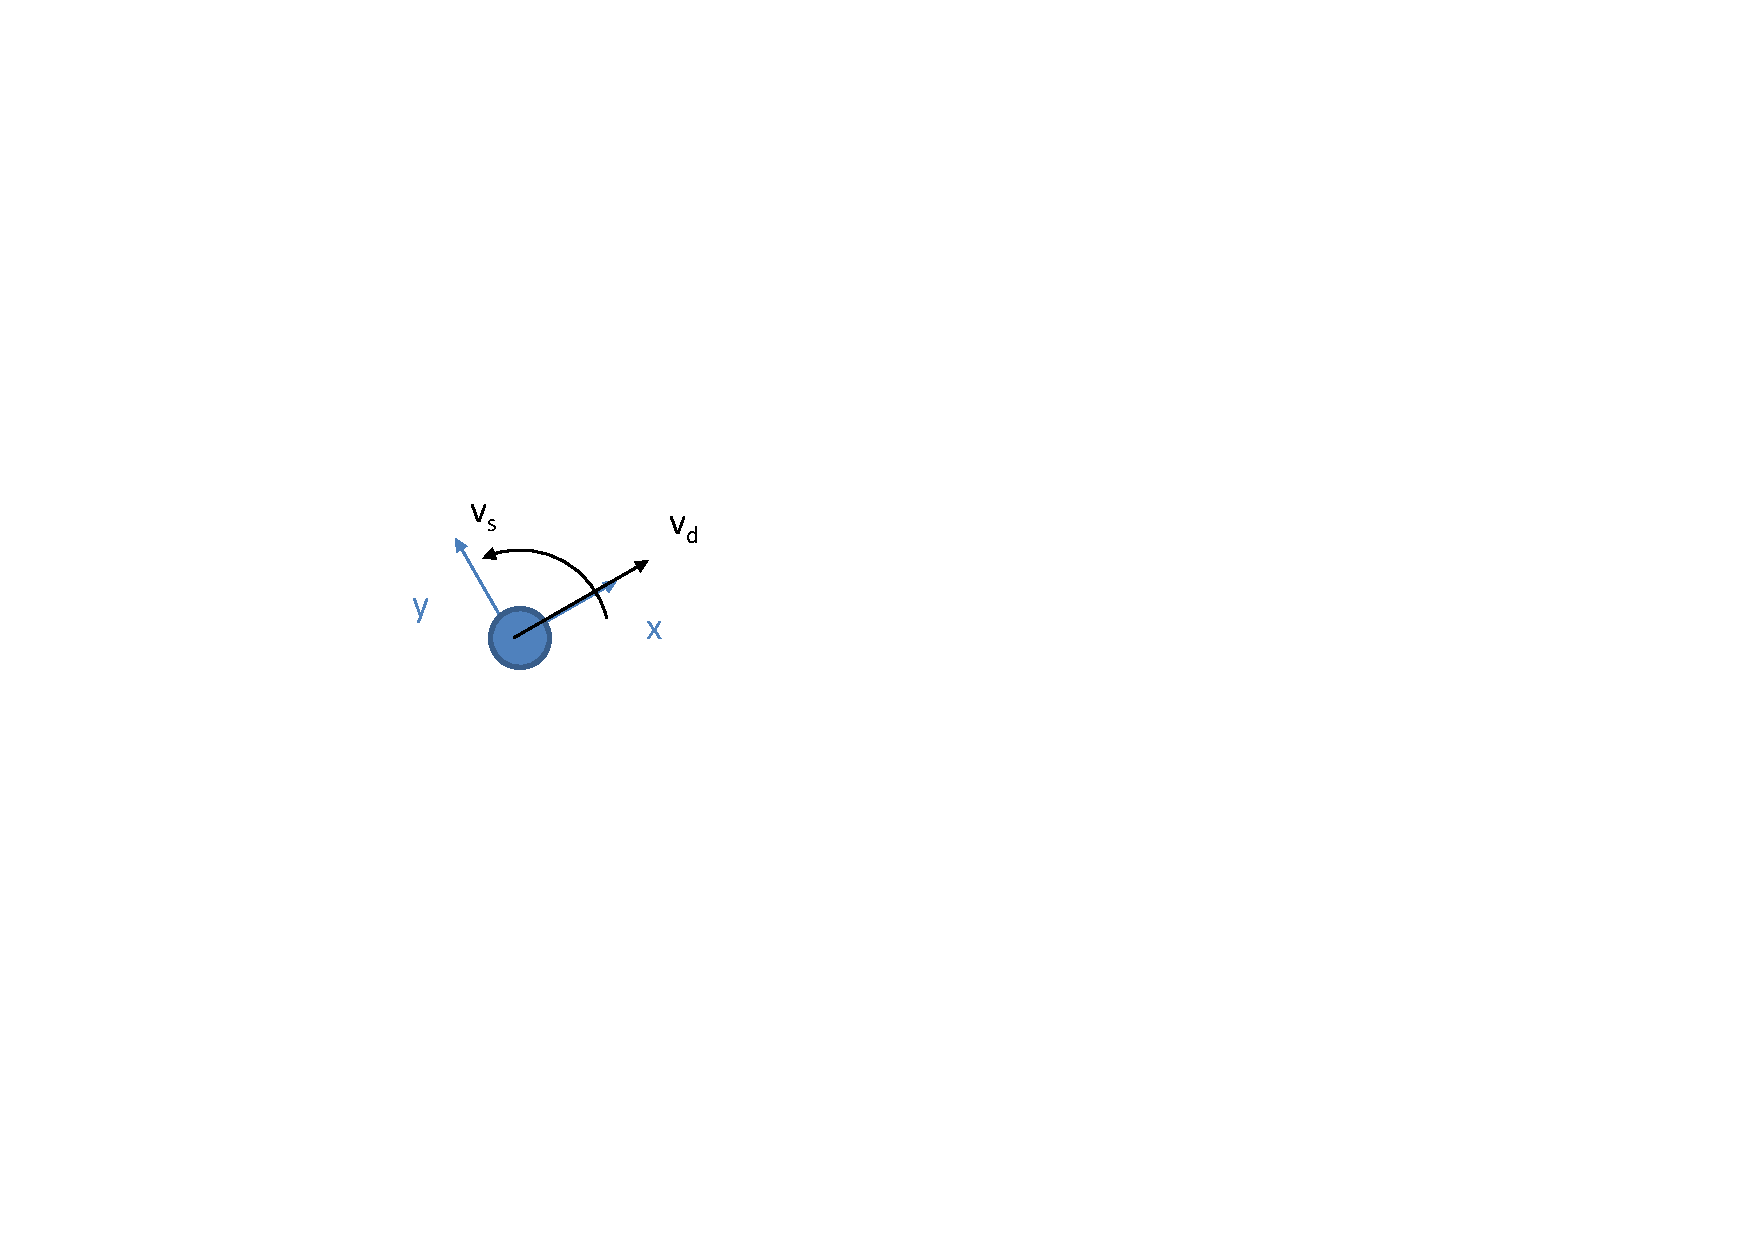
\includegraphics[scale=0.7]{velocidades}\\
  \caption{Velocidad de avance y giro en el sistema de referencia local del robot}\label{fg:velocidades}
\end{figure}


La medida de ángulos se realiza en todo momento en el intervalo [$-\pi$,$\pi$]. Para efectuar la conversión a este rango se utiliza la función \prog{AngRango}.

Como se expuso en el capítulo \ref{ch:estado}, resulta conveniente utilizar un regulador con realimentación que emplee información sobre la posición del robot en cada instante para obtener unos valores de velocidad que permitan llegar al objetivo dado.

Para que el robot se traslade mirando de frente la mayor parte del tiempo, se busca minimizar la diferencia entre su orientación y la del vector que lo une con el punto de destino. Al mismo tiempo el robot deberá irse acercando a dicho punto de destino.

\begin{figure}[bt]
  % Requires \usepackage{graphicx}
  \centering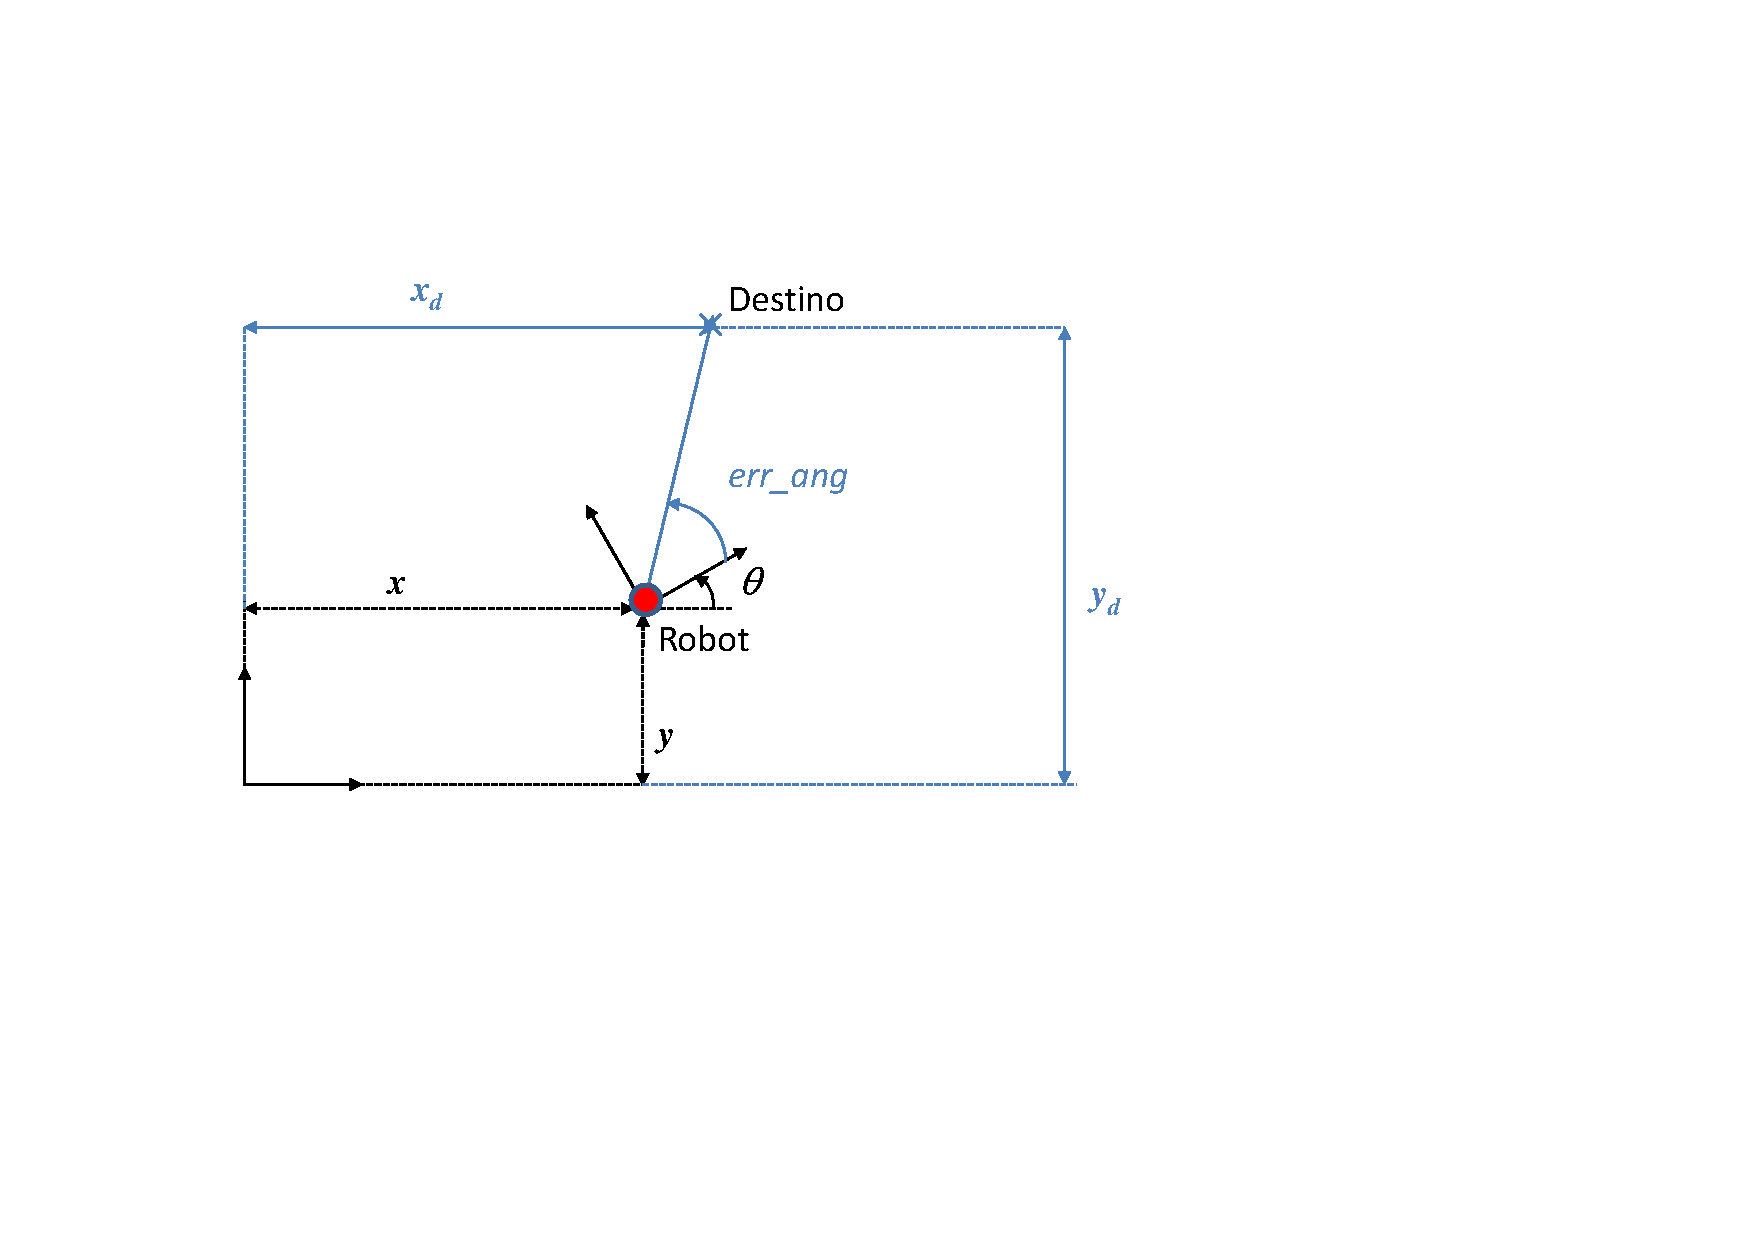
\includegraphics[scale=0.6]{err_ang}\\
  \caption{Control de la orientación del robot}\label{fg:err_ang}
\end{figure}

\begin{figure}[bt]
  % Requires \usepackage{graphicx}
  \centering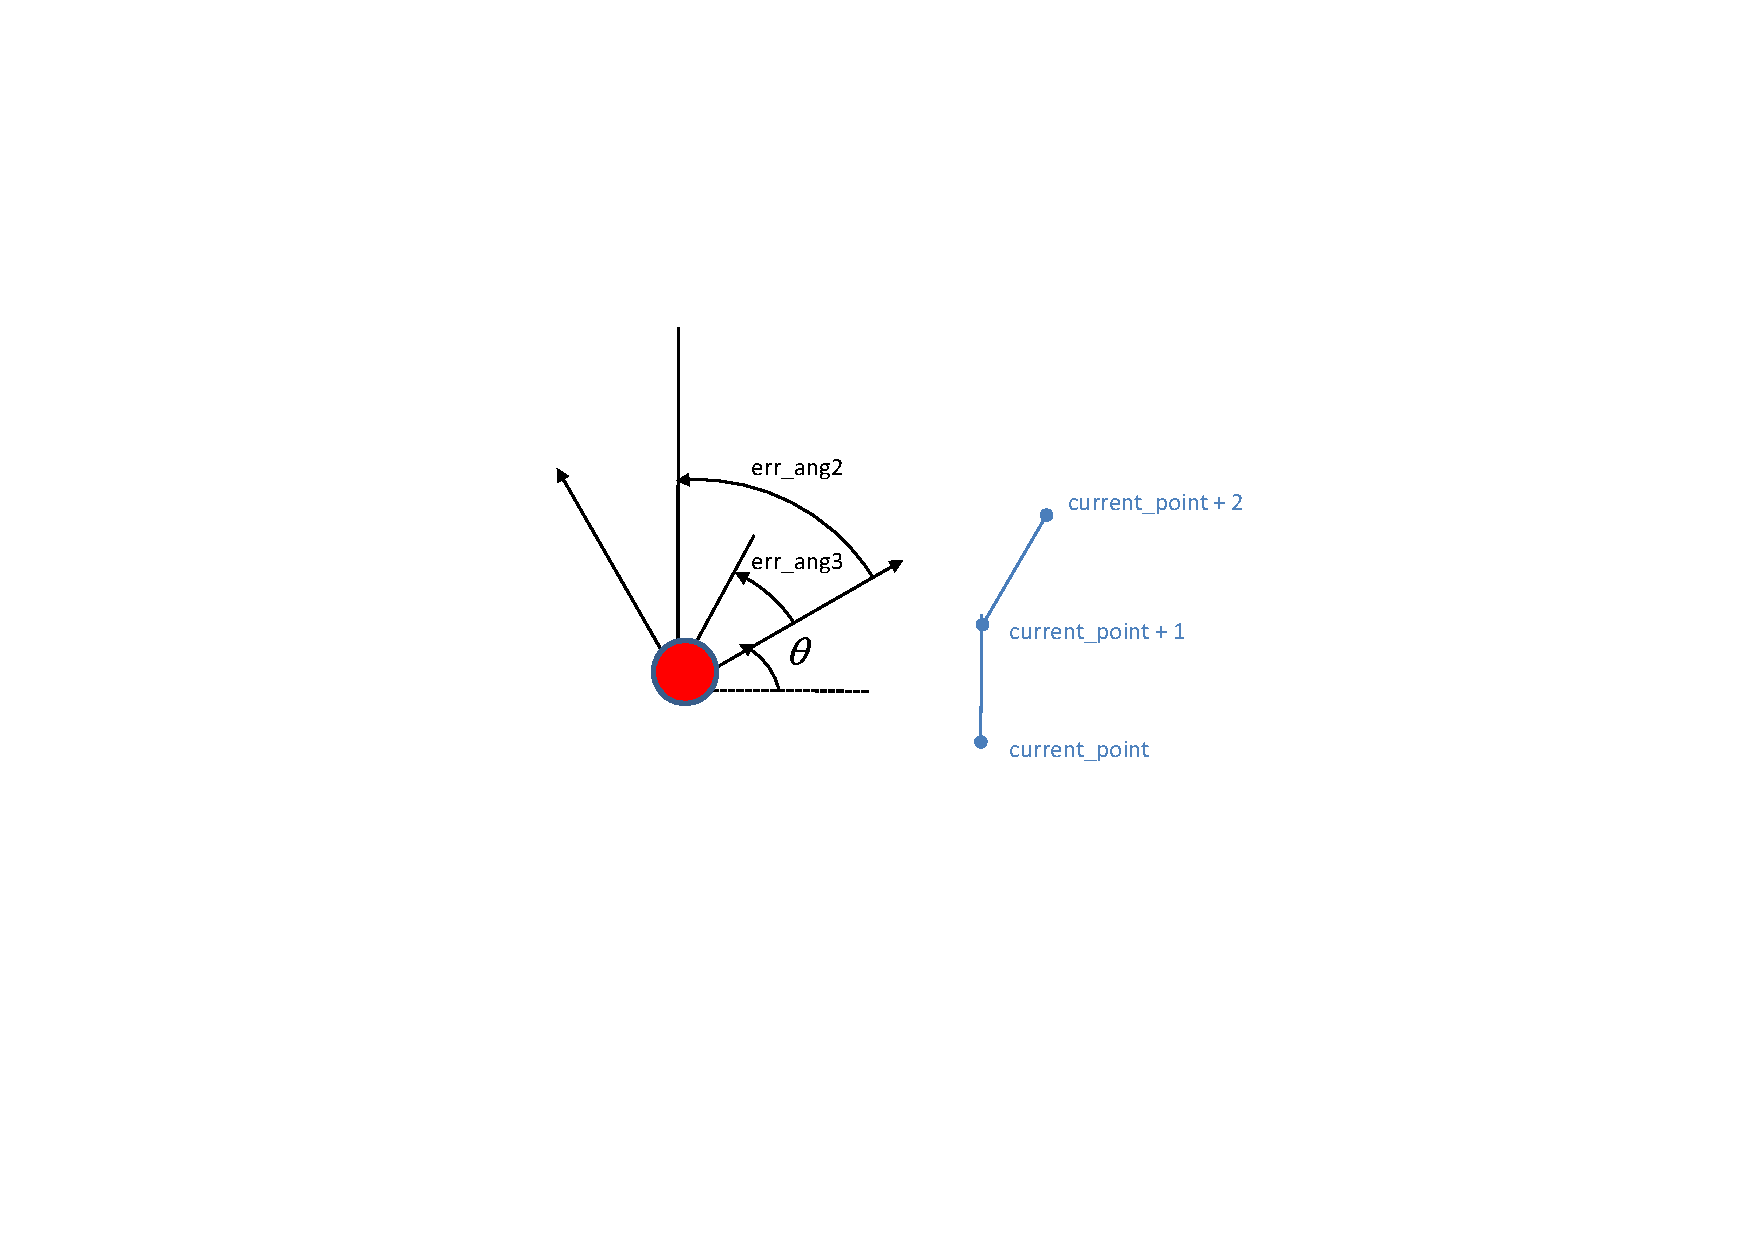
\includegraphics[scale=0.5]{err_ang23}\\
  \caption{Nuevos errores incorporados al regulador}\label{fg:err_ang23}
\end{figure} 

Como puede verse en la figura \ref{fg:err_ang}, el ángulo resultante de esa diferencia de orientaciones se llamará \prog{err\_ang}. En función de su valor se distinguen cuatro casos principales en los cuales se utilizaron en una primera aproximación las ganancias indicadas en el cuadro \ref{vel1}, donde todas las magnitudes están expresadas en el Sistema Internacional salvo cuando se especifica lo contrario.

\begin{table}[hbt]
\begin{center}
\caption{Regulador inicial para el control de movimiento} \label{vel1}

\vspace{5mm}

\begin{tabular}{ll}
\hline\hline
170º$<err\_ang(º)$ \\ \hline
Urbano:      &  Pioneer:   \\
        $v_{d}=0$                   & $v_{d}=0$\\
        $v_{s}=30err\_ang$  & $v_{s}=0.65err\_ang$ \\
\hline
  45º$<err\_ang(º)<$170º \\ \hline
Urbano:  & Pioneer:\\
        $v_{d}=2$                  & $v_{d}=0.025$\\
        $v_{s}=40err\_ang$ & $v_{s}=0.7err\_ang$\\
\hline
15º$<err\_ang(º)<$45º \\ \hline
Urbano:      &  Pioneer:   \\
        $v_{d}=6$                  & $v_{d}=0.1$\\
        $v_{s}=34err\_ang$ & $v_{s}=0.7err\_ang$ \\
\hline
$err\_ang(º)<$15º \\ \hline
Urbano:  & Pioneer: \\
        $v_{d}=10$                & $v_{d}=0.4$\\
        $v_{s}=26err\_ang$ & $v_{s}=0.6err\_ang$\\
\hline\hline
\end{tabular}
\end{center}
\end{table}

Al aumentar la duración del ciclo de tareas cuando se utiliza el robot real Urbano, los comandos de velocidad enviados de acuerdo con el cuadro a \ref{vel1} llegaban con retraso y el robot daba algunos bandazos. Para solucionar este problema se modificó el regulador de forma que se contemplara también la orientación de la trayectoria en el tramo en que se encuentra el robot en cada instante y la orientación en el tramos siguiente, a modo de control predictivo. Los nuevos ángulos sobre los que también se actúa se denominarán \prog{err\_ang2} y \prog{err\_ang3}, respectivamente, y se muestran en la figura \ref{fg:err_ang23}.
 
La acción de control resultante es una combinación lineal de las acciones sobre estos tres ángulos. Se ha utilizado un peso de 0.3 para regular \prog{err\_ang}, un peso de 0.2 para regular \prog{err\_ang2} y un peso de 0.5 para regular \prog{err\_ang3}. El regulador final obtenido utiliza los valores y ganancias que aparecen en el cuadro \ref{vel2}, donde de nuevo las magnitudes se expresan en el S.I. a no ser que se especifique lo contrario. $p1$, $p2$ y $p3$ son los pesos indicados (0.3, 0.2 y 0.5).
Con el robot Pioneer los pesos son los mismos y se mantienen las ganancias del cuadro \ref{vel1}.

\begin{table}[hbt]
\begin{center}
\caption{Regulador para el control de movimiento}
\label{vel2}

\vspace{5mm}

\begin{tabular}{ll}
\hline\hline
160º$<err\_ang(º)$ \\ \hline
Urbano:\\
$v_{d}=0$ \\
$v_{s}=30err\_ang$\\
\hline
  45º$<err\_ang(º)<$160º \\ \hline
Urbano:\\
   $v_{d}=3$ \\
  $v_{s}=p1\times3oerr\_ang + p2\times3oerr\_ang2 + p3\times3oerr\_ang3$ \\
\hline
15º$<err\_ang(º)<$45º \\ \hline
Urbano:\\
$v_{d}=5$ \\
$v_{s}=p1\times26err\_ang + p2\times26err\_ang2 + p3\times26err\_ang3$\\
\hline
$err\_ang(º)<$15º \\ \hline
Urbano: \\
$v_{d}=10$\\
 $v_{s}=p1\times20err\_ang + p2\times26err\_ang2 + p3\times26err\_ang3$\\
\hline\hline
\end{tabular}
\end{center}
\end{table}

El sistema funciona como una máquina de estados. Cuando el robot está lo suficientemente cerca del punto de destino se considera que ha llegado y se establece como destino el siguiente punto de la trayectoria definida. Cuando la distancia al último punto de la misma es menor que 0.5m, actúa un regulador proporcional para que la velocidad de avance del robot vaya disminuyendo gradualmente a medida que se aproxima el final de su recorrido.

Si por algún motivo el robot se halla separado de la trayectoria calculada entre dos puntos, este controlador lo llevaría directamente hacia el punto de destino en línea recta. Esto podría ocasionar el choque con algún obstáculo. Por ello, se utiliza también un regulador que hace que el robot se acerque a la trayectoria definida antes de dirigirse hacia el siguiente punto a alcanzar. Esta situación se muestra en la figura \ref{fg:reg}.

\begin{figure}[h]
  % Requires \usepackage{graphicx}
  \centering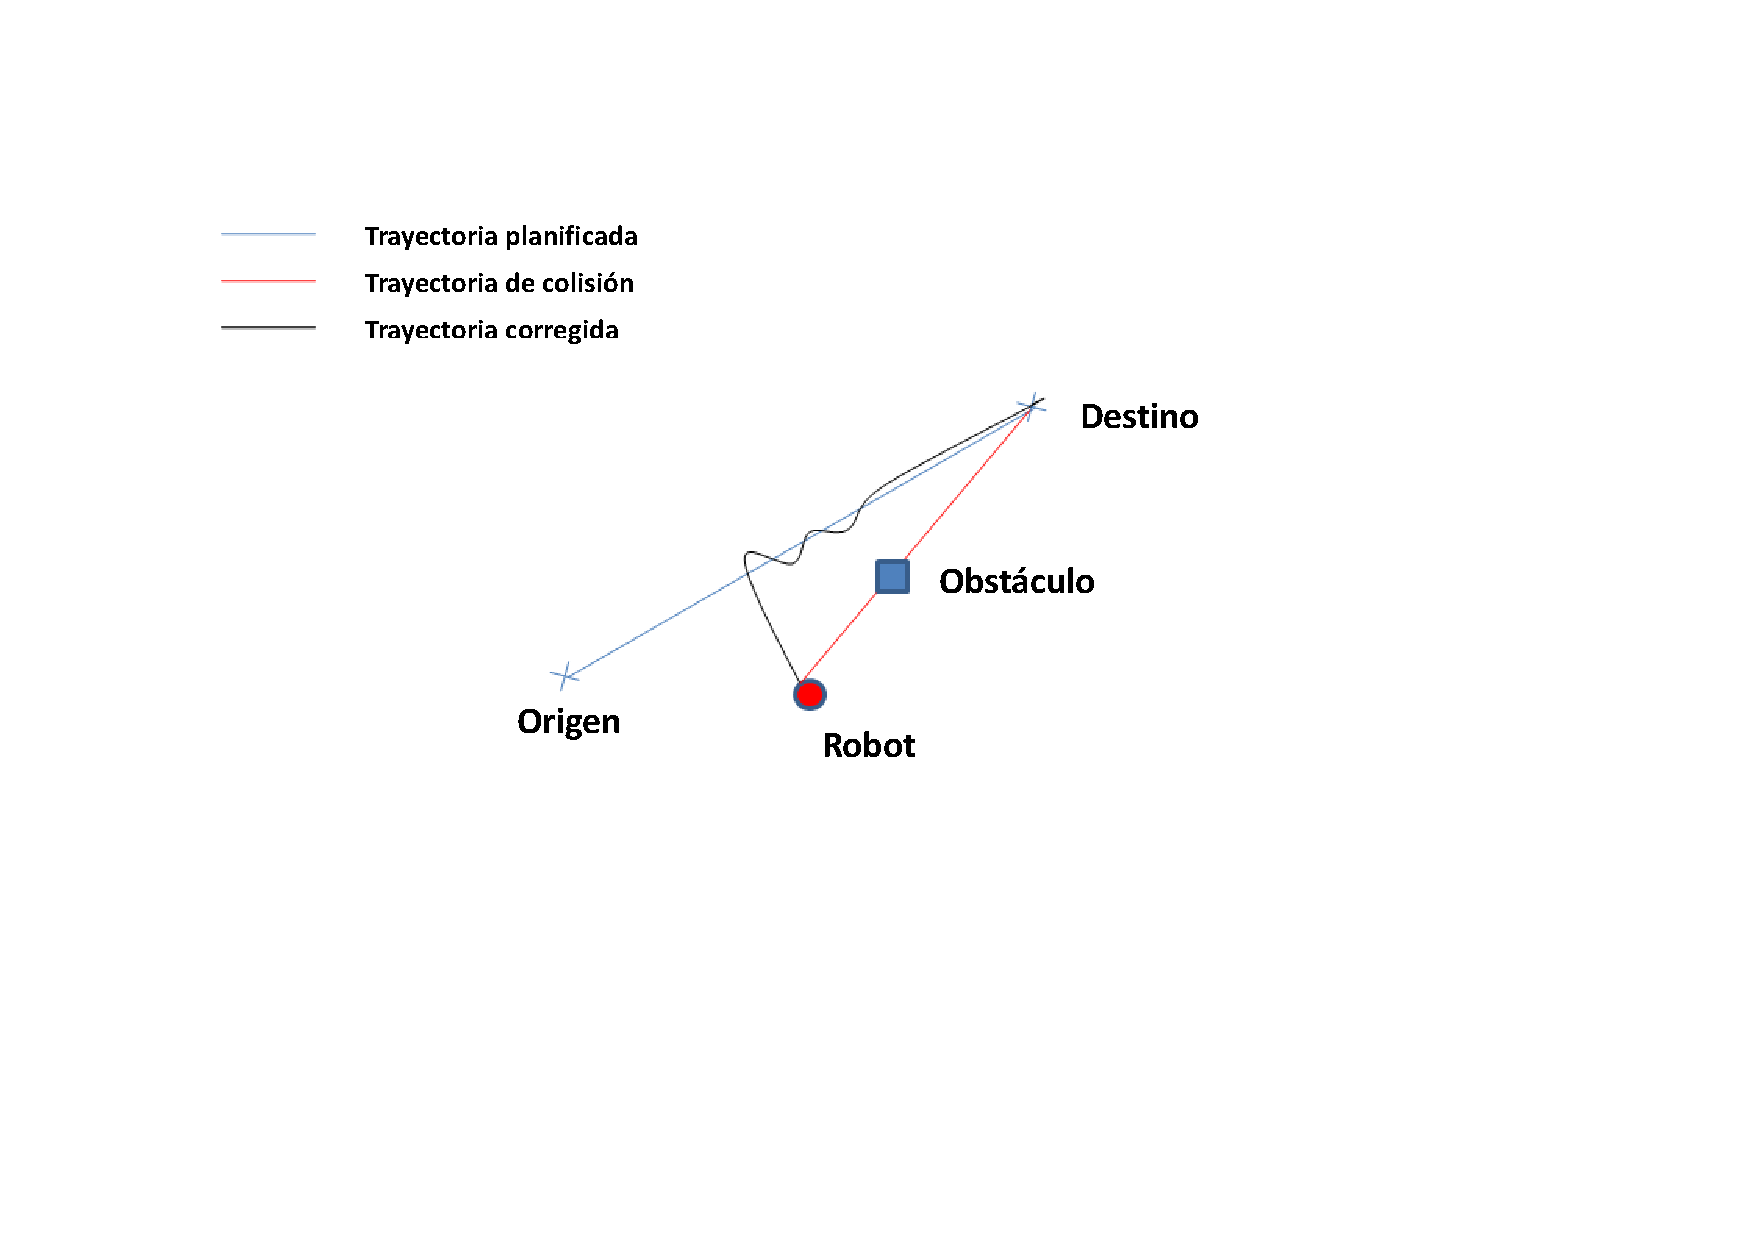
\includegraphics[scale=0.6]{reg}\\
  \caption{Diferentes trayectorias entre dos puntos}\label{fg:reg}
\end{figure}

El algoritmo empleado en este caso requiere medir en primer lugar la distancia de la posición del robot a la recta que une los dos puntos de la trayectoria entre los que se encuentra. Esta distancia tendrá signo positivo o negativo dependiendo de a qué lado de la trayectoria se encuentre el robot (figura \ref{fg:dist2tray}).

\begin{figure}[h]
  % Requires \usepackage{graphicx}
  \centering{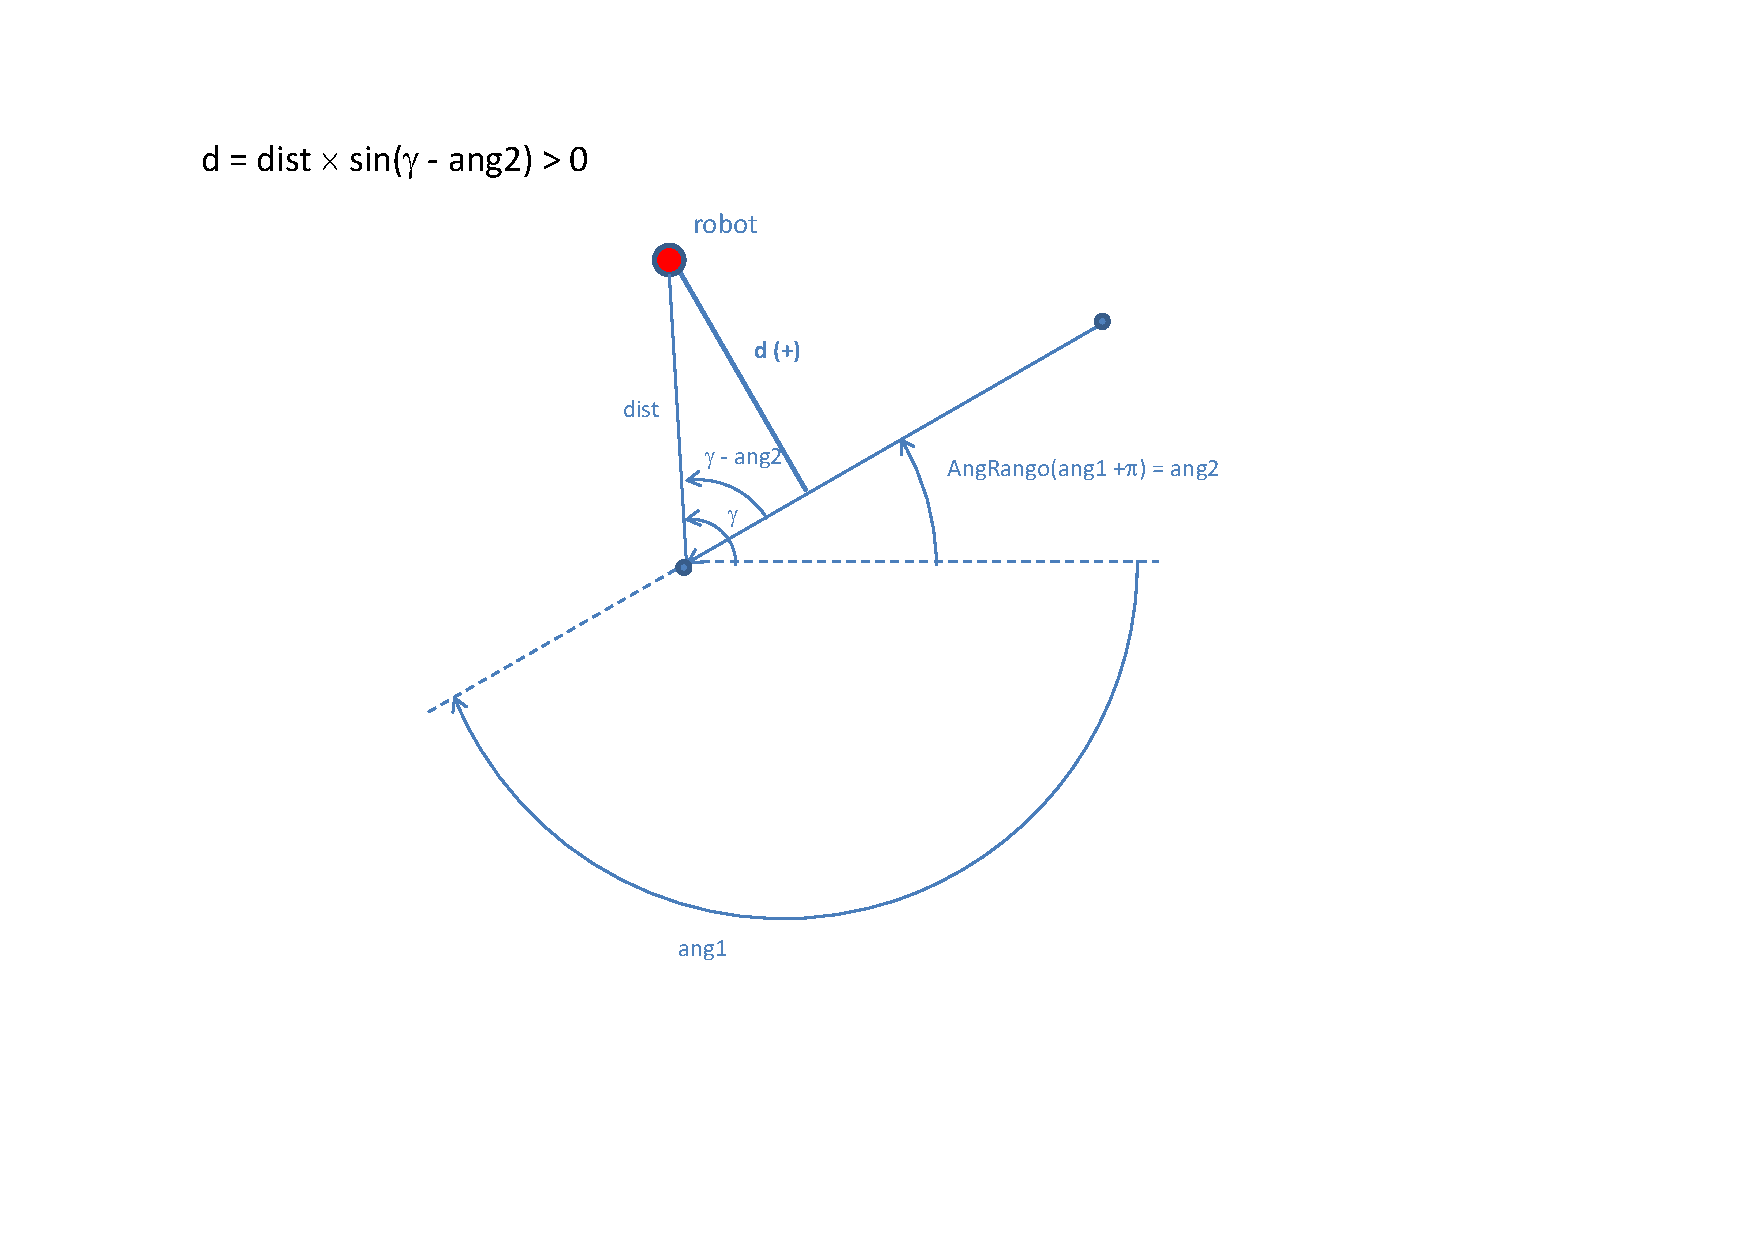
\includegraphics[scale=0.6]{dist2tray}
  \vspace{0.2cm}
   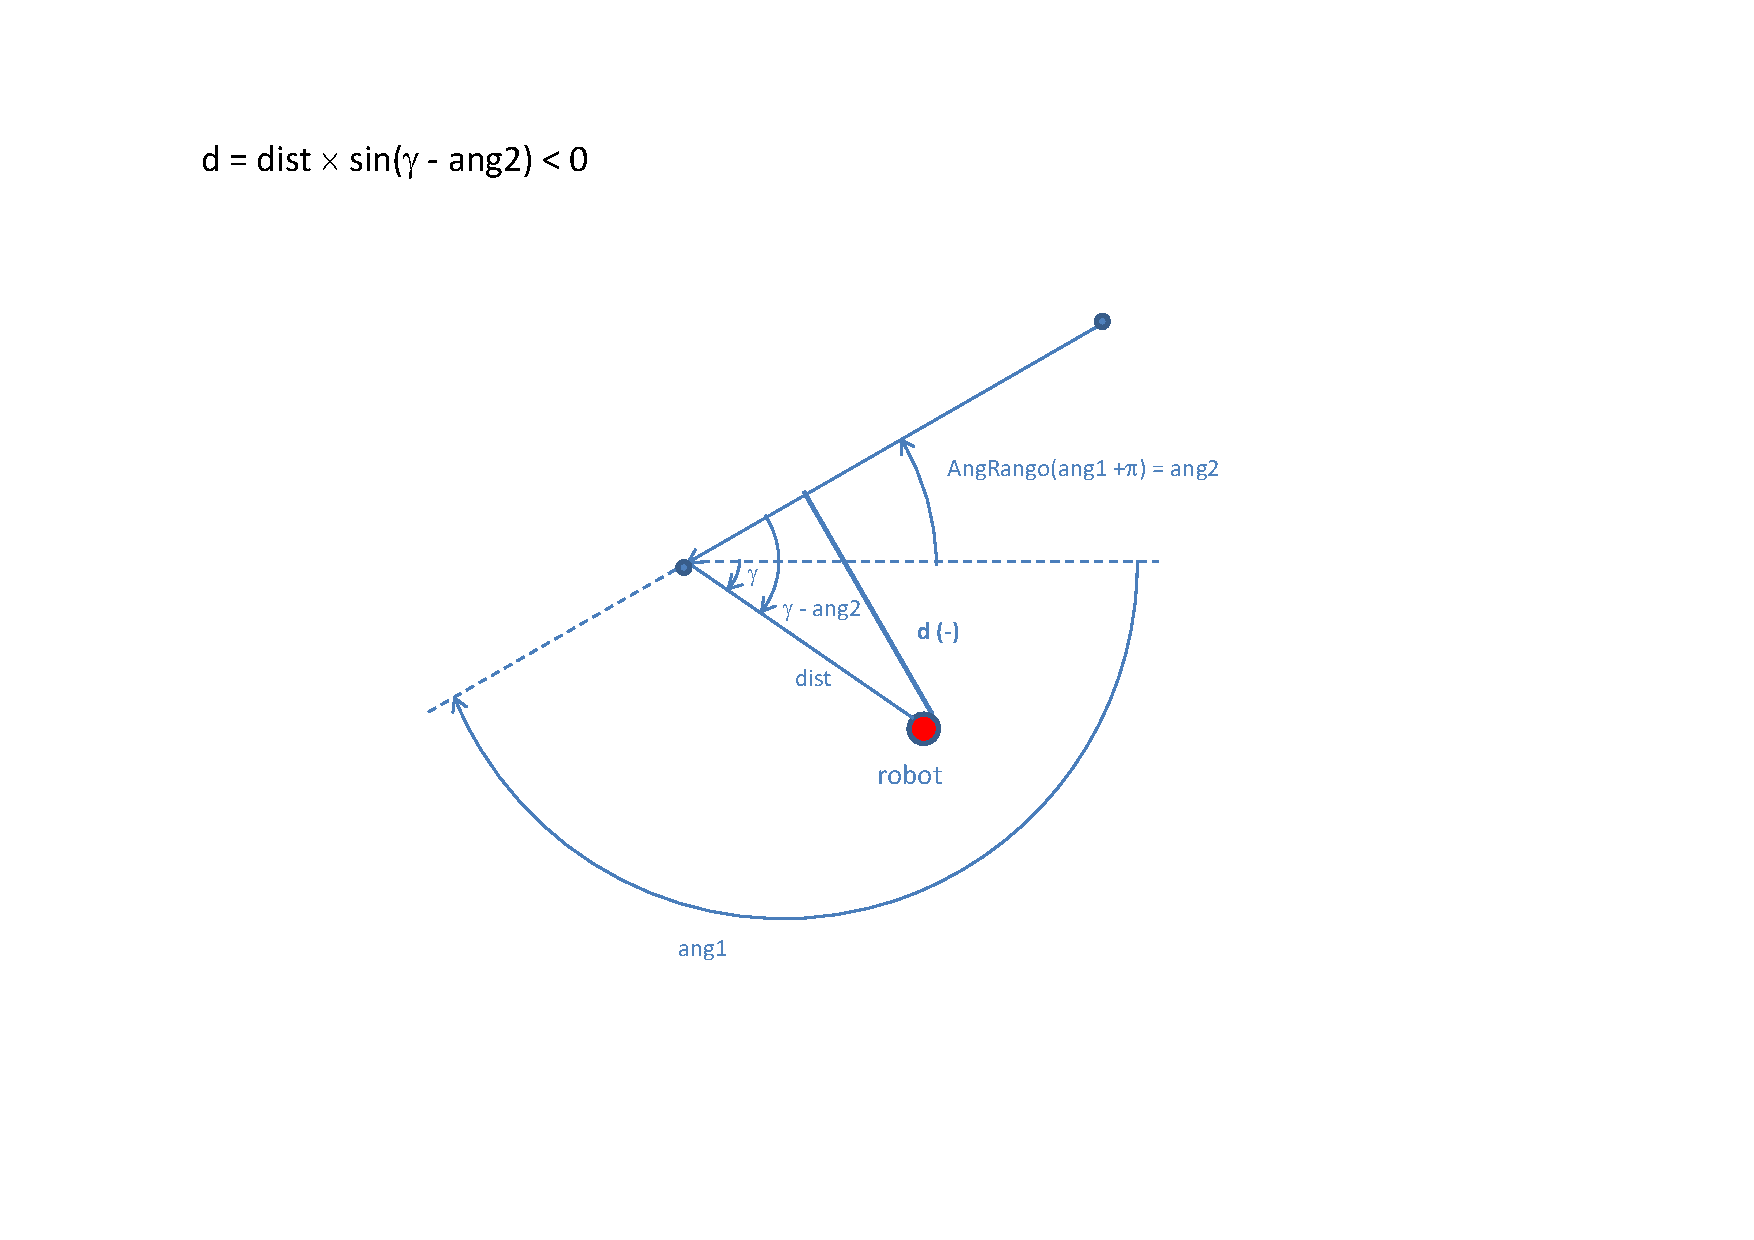
\includegraphics[scale=0.6]{dist2tray2}}  \\
  \caption{ Medida de la distancia del robot al segmento de trayectoria en el que se halla}\label{fg:dist2tray}
\end{figure}

\clearpage

Si el robot está más lejos de la trayectoria que lo establecido por un cierto valor límite, se realizará un control que tienda a dirigirlo perpendicularmente hacia la misma. Para ello se utilizan unos valores de ganancia muy similares a los indicados en la tabla anterior, pero el ángulo que se mide es aquél que separa la orientación del robot con la que debería tener para acercarse perpendicularmente al segmento de trayectoria correspondiente. El modo en que se calcula este ángulo en dos casos en que el robot está situado a un lado u otro de un mismo segmento se muestra en la figura \ref{fg:regu}.

\begin{figure}[hbt]
  % Requires \usepackage{graphicx}
  \centering{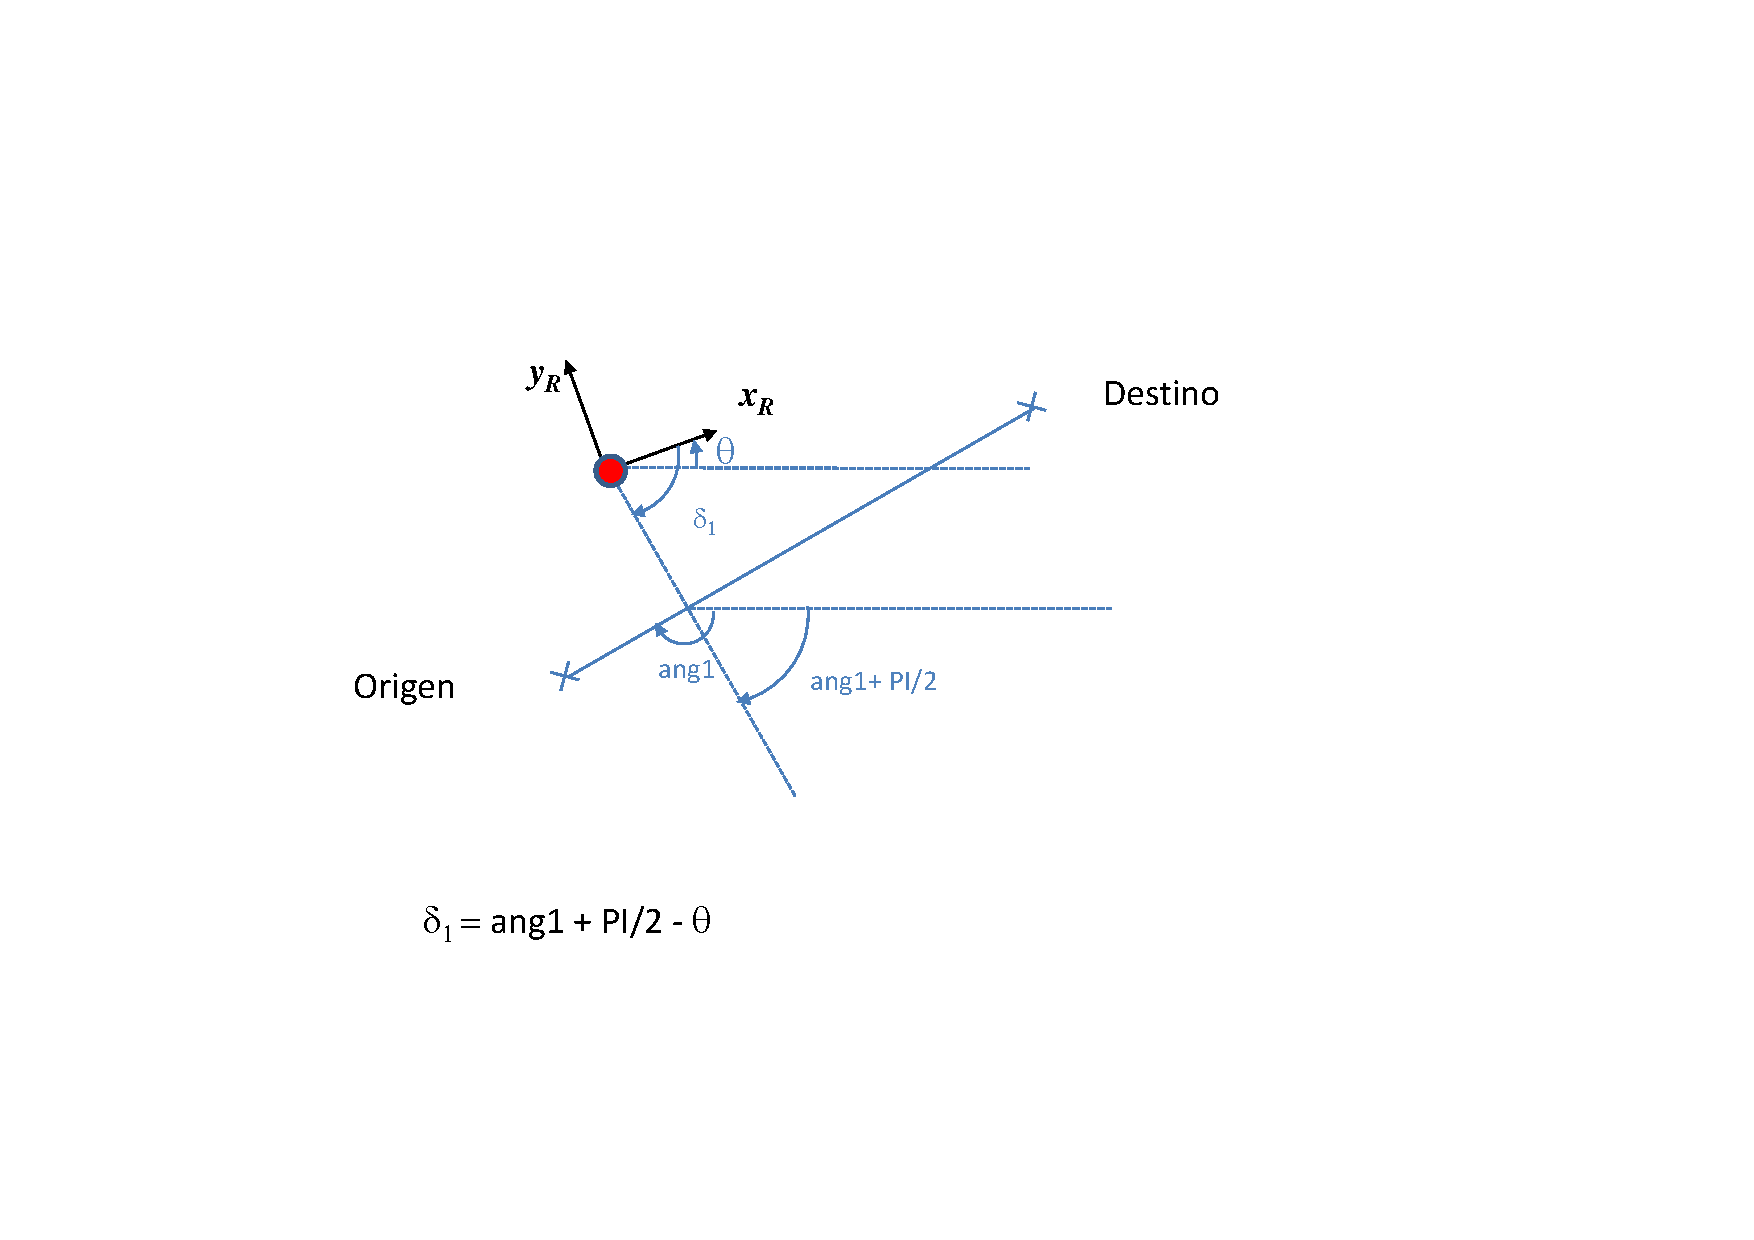
\includegraphics[scale=0.5]{regu1}
  \vspace{0.5cm} 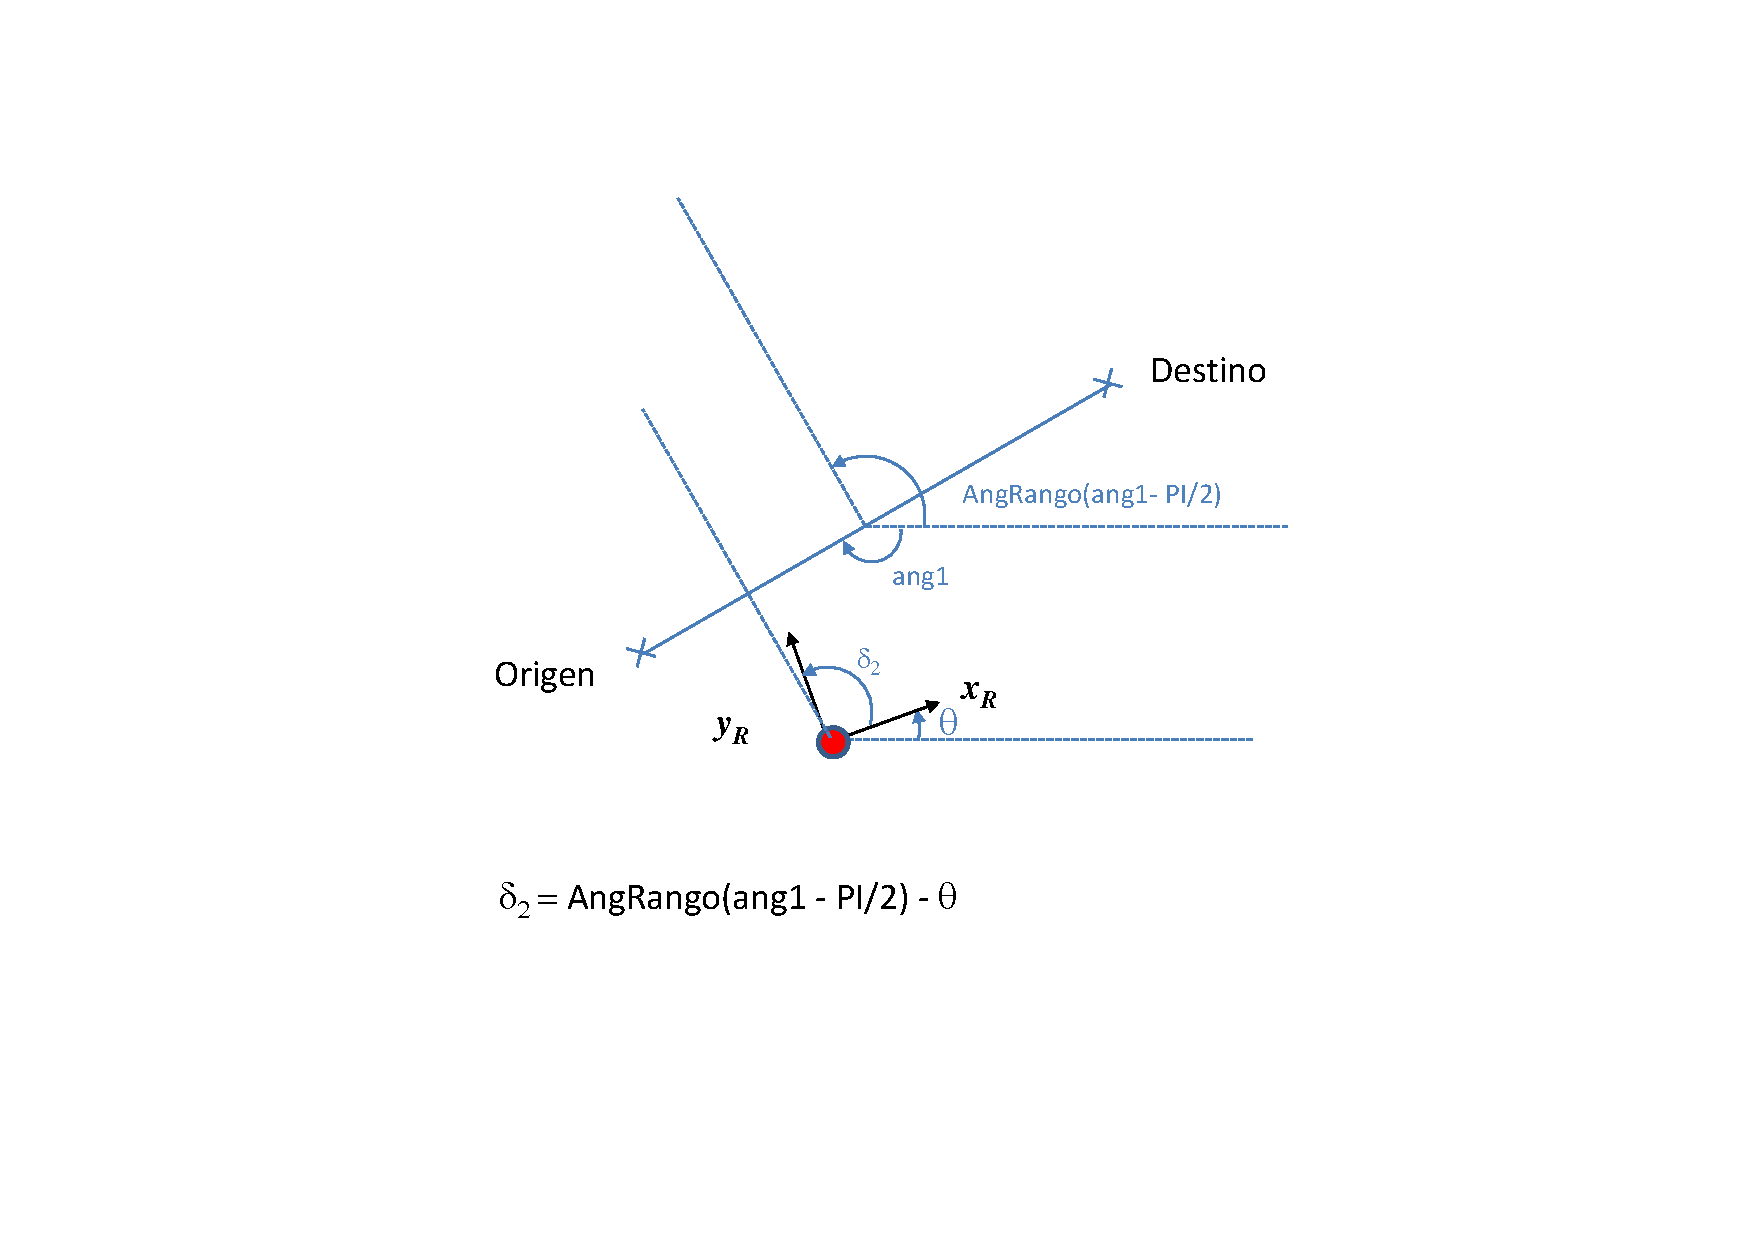
\includegraphics[scale=0.5]{regu2}}  \\
  \caption{Ángulo a regular para que el robot se aproxime a la trayectoria definida en dos casos diferentes}\label{fg:regu}
\end{figure}

\clearpage
Otro aspecto que se tiene en cuenta en el diseño del regulador es el hecho de que el robot pueda pasarse de algún punto de la trayectoria al hallarse muy próximos unos puntos a otros y ser la velocidad alta. En ese caso resultaría absurdo que el robot regresara a dicho punto para seguir la secuencia exacta. Es más conveniente que se dirija hacia aquél que, estando relativamente cerca del destino teórico, sea más cercano al robot. Lo mismo ocurre si la tolerancia que determina si se ha llegado o no a un punto es excesivamente pequeña. Para ello, cada vez que se van a calcular unas nuevas velocidades se busca si en la trayectoria hay algún punto entre los cinco siguientes al punto de destino que se encuentre a menos distancia de la posición del robot que éste.

\section{Planificación de trayectorias}\label{tray}

Como se ha visto en la sección anterior, el control de movimiento del robot precisa disponer de un conjunto de puntos de paso que se vayan definiendo como destinos sucesivos, conformando la trayectoria que ha de seguirse. El alcance de este proyecto no incluye la generación automática de dichos puntos de paso a partir de un destino final dentro de un mapa. Lo que puede hacerse es seleccionar la serie de puntos que determina la trayectoria mediante uso del ratón sobre la interfaz gráfica en la que se ve un mapa o parte de uno. Otra posibilidad para obtener los puntos de la trayectoria consiste en llevar el robot hacia un sitio en modo teleoperado e ir guardando su posición cada vez que recorre una cierta distancia de forma que puede regresar al punto del que partió de manera autónoma.

Cuando los puntos que dan lugar a la trayectoria están bastante separados conviene suavizar los cambios de dirección en la misma. El algoritmo utilizado para ello se explica a continuación.

Mientras sea posible, para cada punto de la trayectoria se toma el siguiente a él como base o punto intermedio a suprimir en caso necesario. Se definen dos vectores que van desde la base hasta el punto anterior y hasta el punto siguiente a ella, respectivamente, y se mide el ángulo que los separa. Si este ángulo, que llamaremos erro\_ang, es menor que 20º o superior a 160º no ha de redondearse la trayectoria; simplemente se pasa al siguiente de sus puntos. En caso contrario se halla su bisectriz para situar sobre ella el centro del arco de circunferencia que servirá para suavizar la trayectoria en el punto base. A partir del centro se irán determinando puntos de forma que su distancia a él sea igual al radio y que queden uniformemente repartidos sobre un arco tangente a los dos segmentos de trayectoria que se unen. El cálculo de los ángulos que permiten calcular las coordenadas de los puntos del arco se basa en un ángulo auxiliar definido como \prog{alfa\_ref} = \prog{AngRango}$(\pi - ang\_bis)$ y es diferente según \prog{erro\_ang} sea positivo o negativo, dado que esto condiciona el sentido en que deben ir creciendo dichos ángulos.

\begin{figure}[bt]
  % Requires \usepackage{graphicx}
  \centering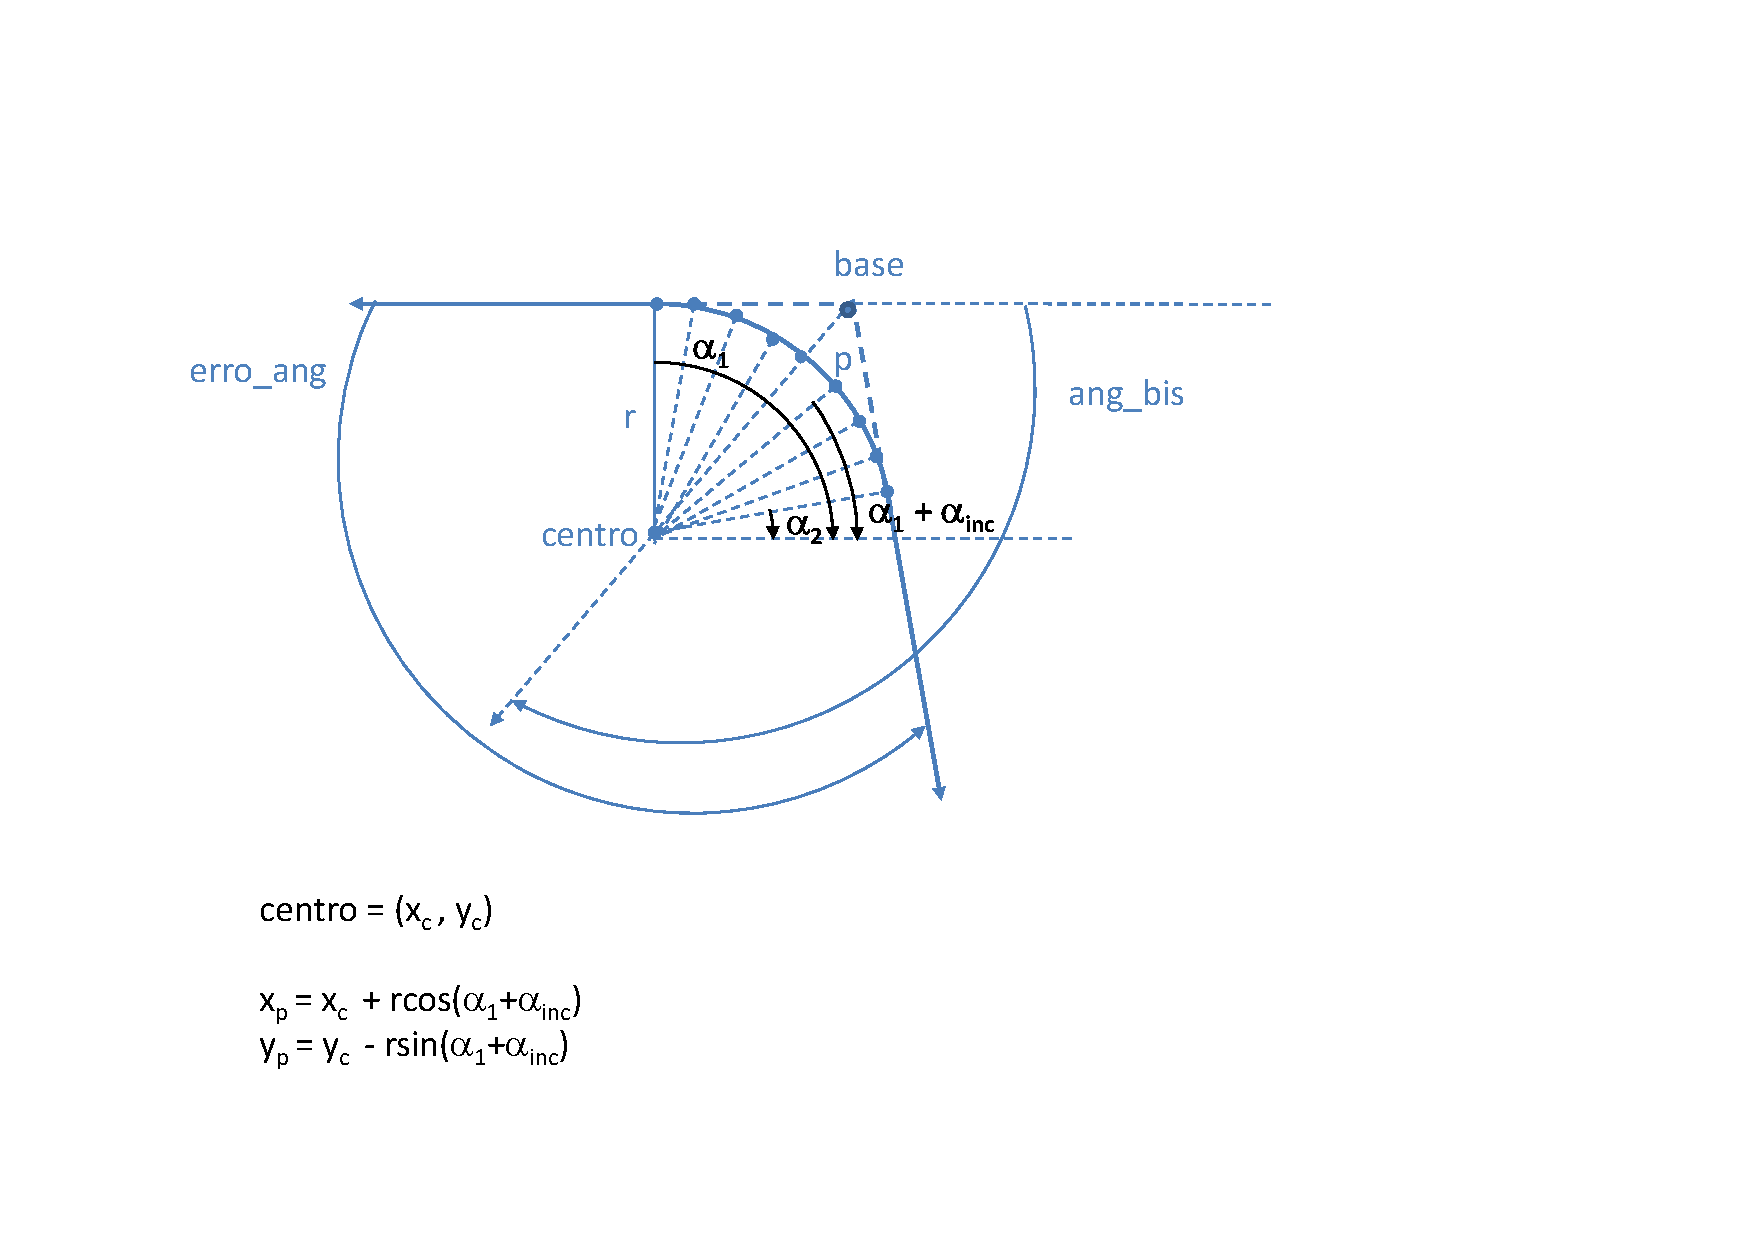
\includegraphics[scale=0.6]{smooth}\\
  \caption{Cálculo de coordenadas de los puntos del arco con 
  $\mbox{erro\_ang} > 0$}\label{fg:smooth}
\end{figure}

En la figura \ref{fg:smooth} se muestra un caso en el que \prog{erro\_ang} es mayor que cero. Para la obtención de los sucesivos puntos el valor de $ang_{inc}$ se va incrementando en 0.1 rad mientras que al sumarse a $\alpha_{1}$ no se sobrepase el valor de $\alpha_{2}$. Estos dos ángulos vienen dados por:

\begin{eqnarray*}
\alpha_{1}  & = & \mbox{AngRango} \left ( alpha\_ref - 
   \left (\frac{\pi}{2} - \frac{\mbox{erro\_ang}}{2} \right ) \right )\\
 \alpha_{2}  & = & \mbox{AngRango} \left ( alpha\_ref + 
   \left (\frac{\pi}{2} - \frac{\mbox{erro\_ang}}{2} \right ) \right )\\
\end{eqnarray*}

Así, para la trayectoria de la figura \ref{fg:smooth} los valores son:
\begin{eqnarray*}
\mbox{erro\_ang}  & = & 100º \\
\mbox{alfa\_ref}     &=  & \mbox{AngRango} (\pi - (-130º))\\
                                  & = &\mbox{AngRango} (310º) \\
                                  & = & -50º\\
alpha_{1}                &= & \mbox{AngRango} (-50º - 90º + 50º)\\ 
                                 & = & \mbox{AngRango} (-90º)\\
                                 & = & -90º\\ 
alpha_{2}                &= & \mbox{AngRango} (-50º + 90º - 50º)\\ 
                                 & = & \mbox{AngRango} (-10º)\\
                                 & = & -10º\\                             
\end{eqnarray*}



Si \prog{erro\_ang} es menor que cero, los ángulos extremos mediante los cuales se calculan las coordenadas de los puntos del arco son:

\begin{eqnarray*}
\alpha_{1}  & = & \mbox{AngRango} \left ( alpha\_ref + 
   \left (\frac{\pi}{2} + \frac{\mbox{erro\_ang}}{2} \right ) \right )\\
 \alpha_{2}  & = & \mbox{AngRango} \left ( alpha\_ref - 
   \left (\frac{\pi}{2} + \frac{\mbox{erro\_ang}}{2} \right ) \right )\\
\end{eqnarray*}

Ahora el ángulo $\alpha_{dec}$, figura \ref{fg:smooth2}, se va decrementando 0.1 rad hasta que su suma con $\alpha_{1}$ se hace menor que $\alpha_{2}$.

\begin{figure}[hbt]
  % Requires \usepackage{graphicx}
  \centering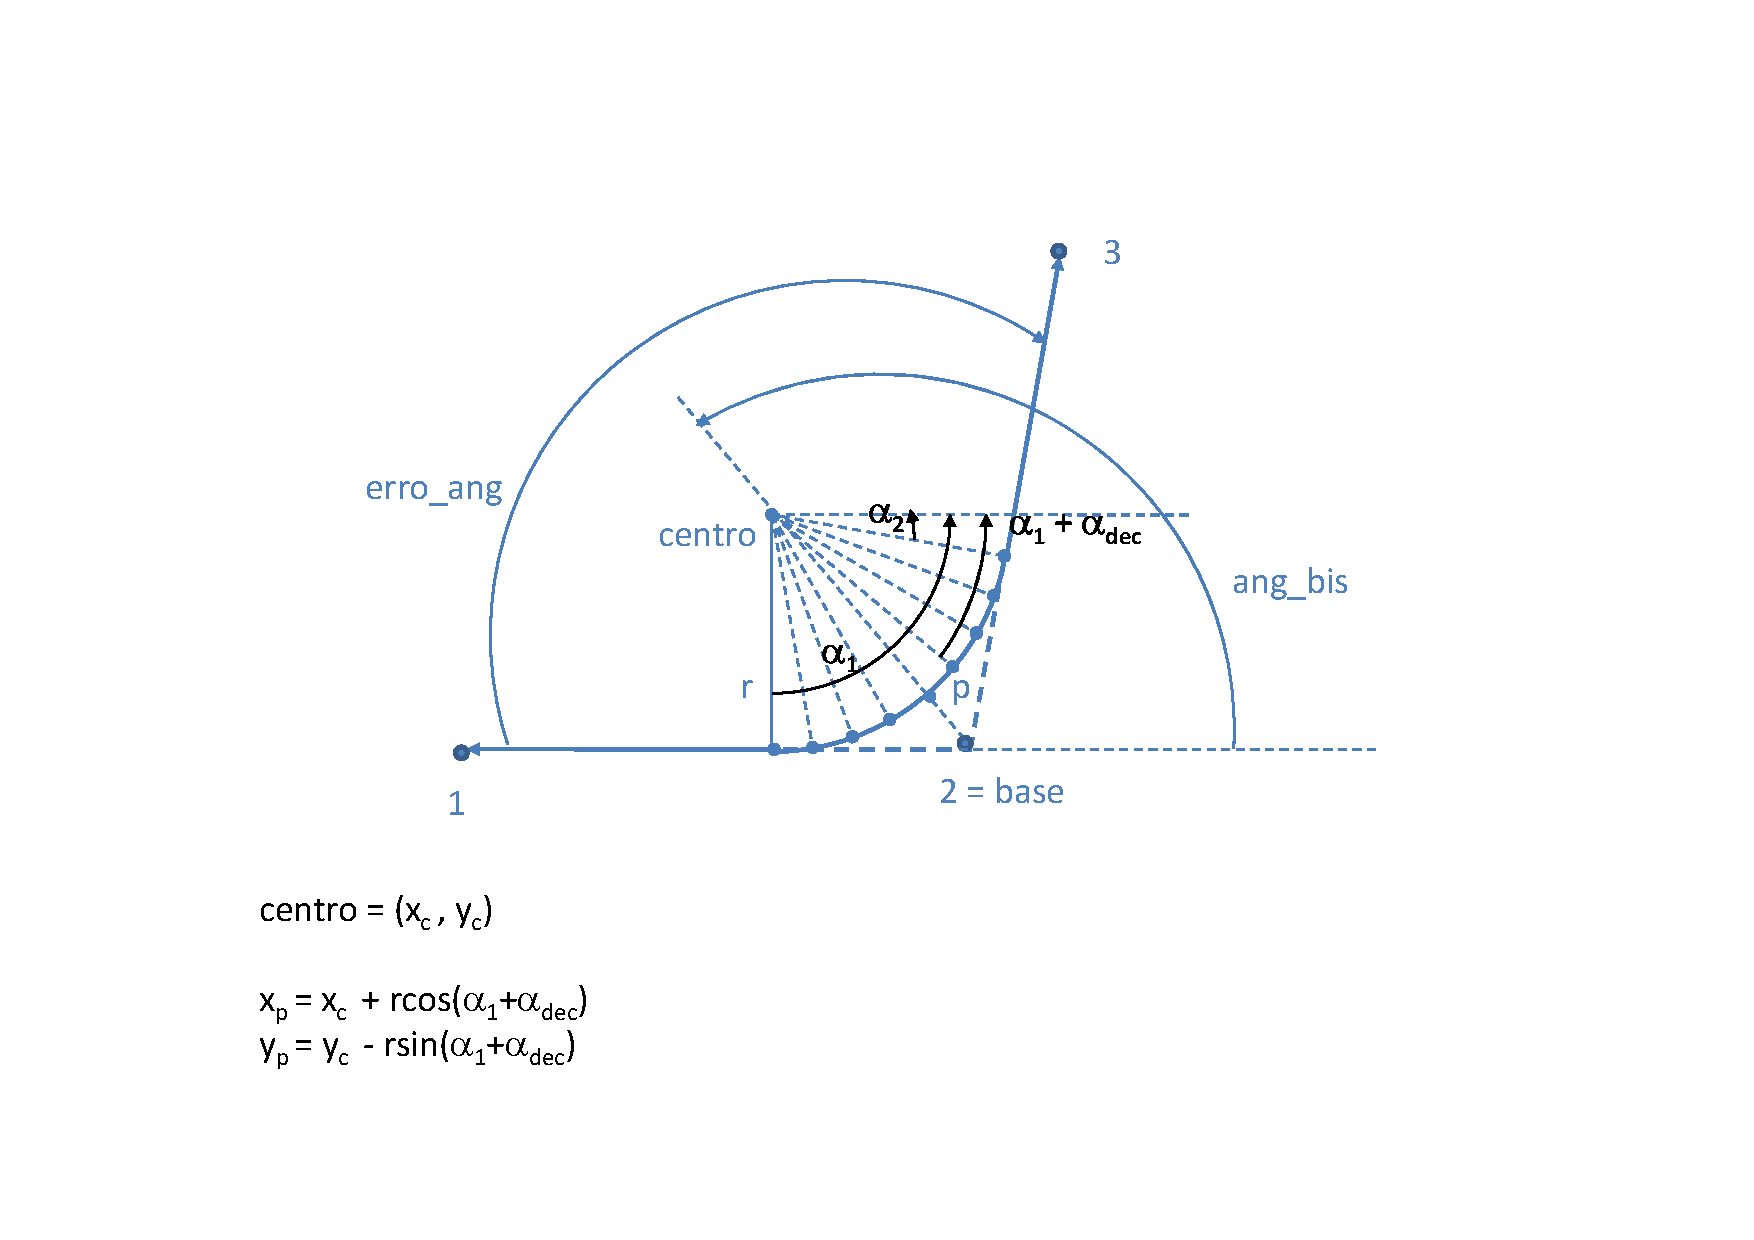
\includegraphics[scale=0.6]{smooth2}\\
  \caption{Cálculo de coordenadas de los puntos del arco con erro\_ang $< 0$}\label{fg:smooth2}
\end{figure}

En el caso concreto representado en la figura \ref{fg:smooth2} los ángulos que se muestran toman los siguientes valores:
\begin{eqnarray*}
\mbox{erro\_ang}  & = & -100º \\
\mbox{alfa\_ref}     &=  & \mbox{AngRango} (\pi - 130º)\\
                                  & = &\mbox{AngRango} (50º) \\
                                  & = & 50º\\
alpha_{1}                &= & \mbox{AngRango} (50º + 90º - 50º)\\ 
                                 & = & \mbox{AngRango} (-90º)\\
                                 & = & -90º\\ 
alpha_{2}                &= & \mbox{AngRango} (50º - 90º + 50º)\\ 
                                 & = & \mbox{AngRango} (-10º)\\
                                 & = & 10º\\                             
\end{eqnarray*}

\clearpage

A continuación se muestra el resultado de aplicar el sistema implementado a diferentes trayectorias. Como puede verse, el color negro representa la trayectoria original y el azul, la trayectoria suavizada. El valor del radio utilizado es 1m.

\begin{figure}[hbt]
  % Requires \usepackage{graphicx}
  \centering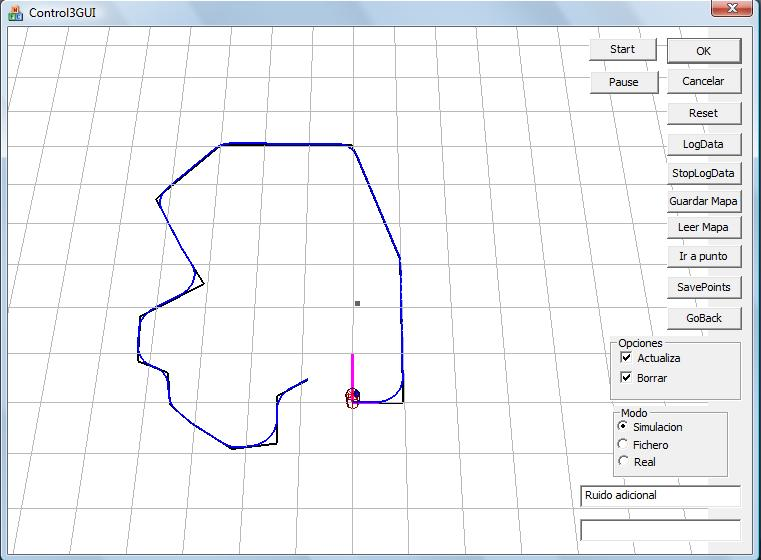
\includegraphics[scale=0.5]{SmoothT}\\
  \vspace{0.2cm}
  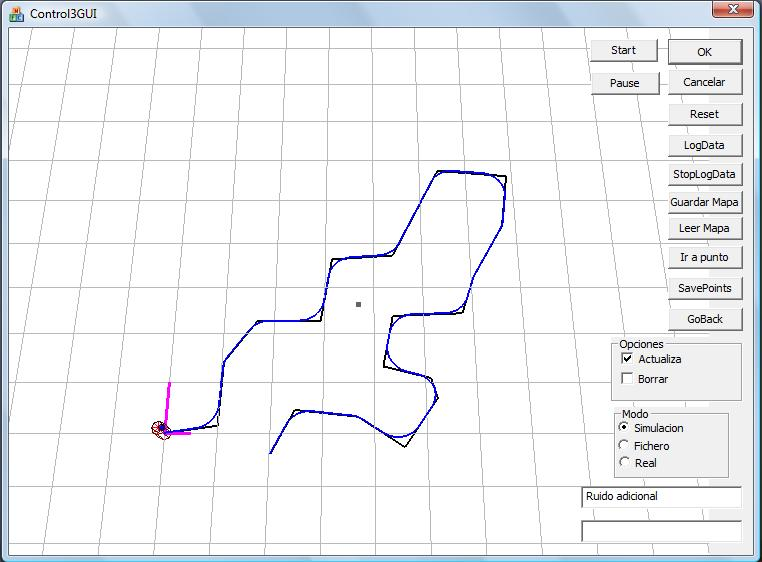
\includegraphics[scale=0.5]{SmoothT2}\label{fg:smoothT}
  \caption{Trayectorias suaves conseguidas}
\end{figure}

\section{Control Reactivo}\label{reactivo}

Una trayectoria planificada y modificada de acuerdo con los apartados anteriores puede requerir nuevos cambios si se detectan obstáculos cercanos a ella. Este aspecto se contempla en el proyecto a través de de un algoritmo que desvía los puntos de la trayectoria cercanos a los objetos. Para cada punto $i$ de la trayectoria nominal se siguen los mismos pasos. En primer lugar, se define un punto $p$ sobre la perpendicular al segmento que une ese punto de la trayectoria con el siguiente de forma que su distancia a dicho punto de la trayectoria sea 1m (ver figura \ref{fg:elastic}). El vector que une el punto de la trayectoria con el punto $p$ se denominará $v_{1}$.

\begin{figure}[hbt]
  % Requires \usepackage{graphicx}
  \centering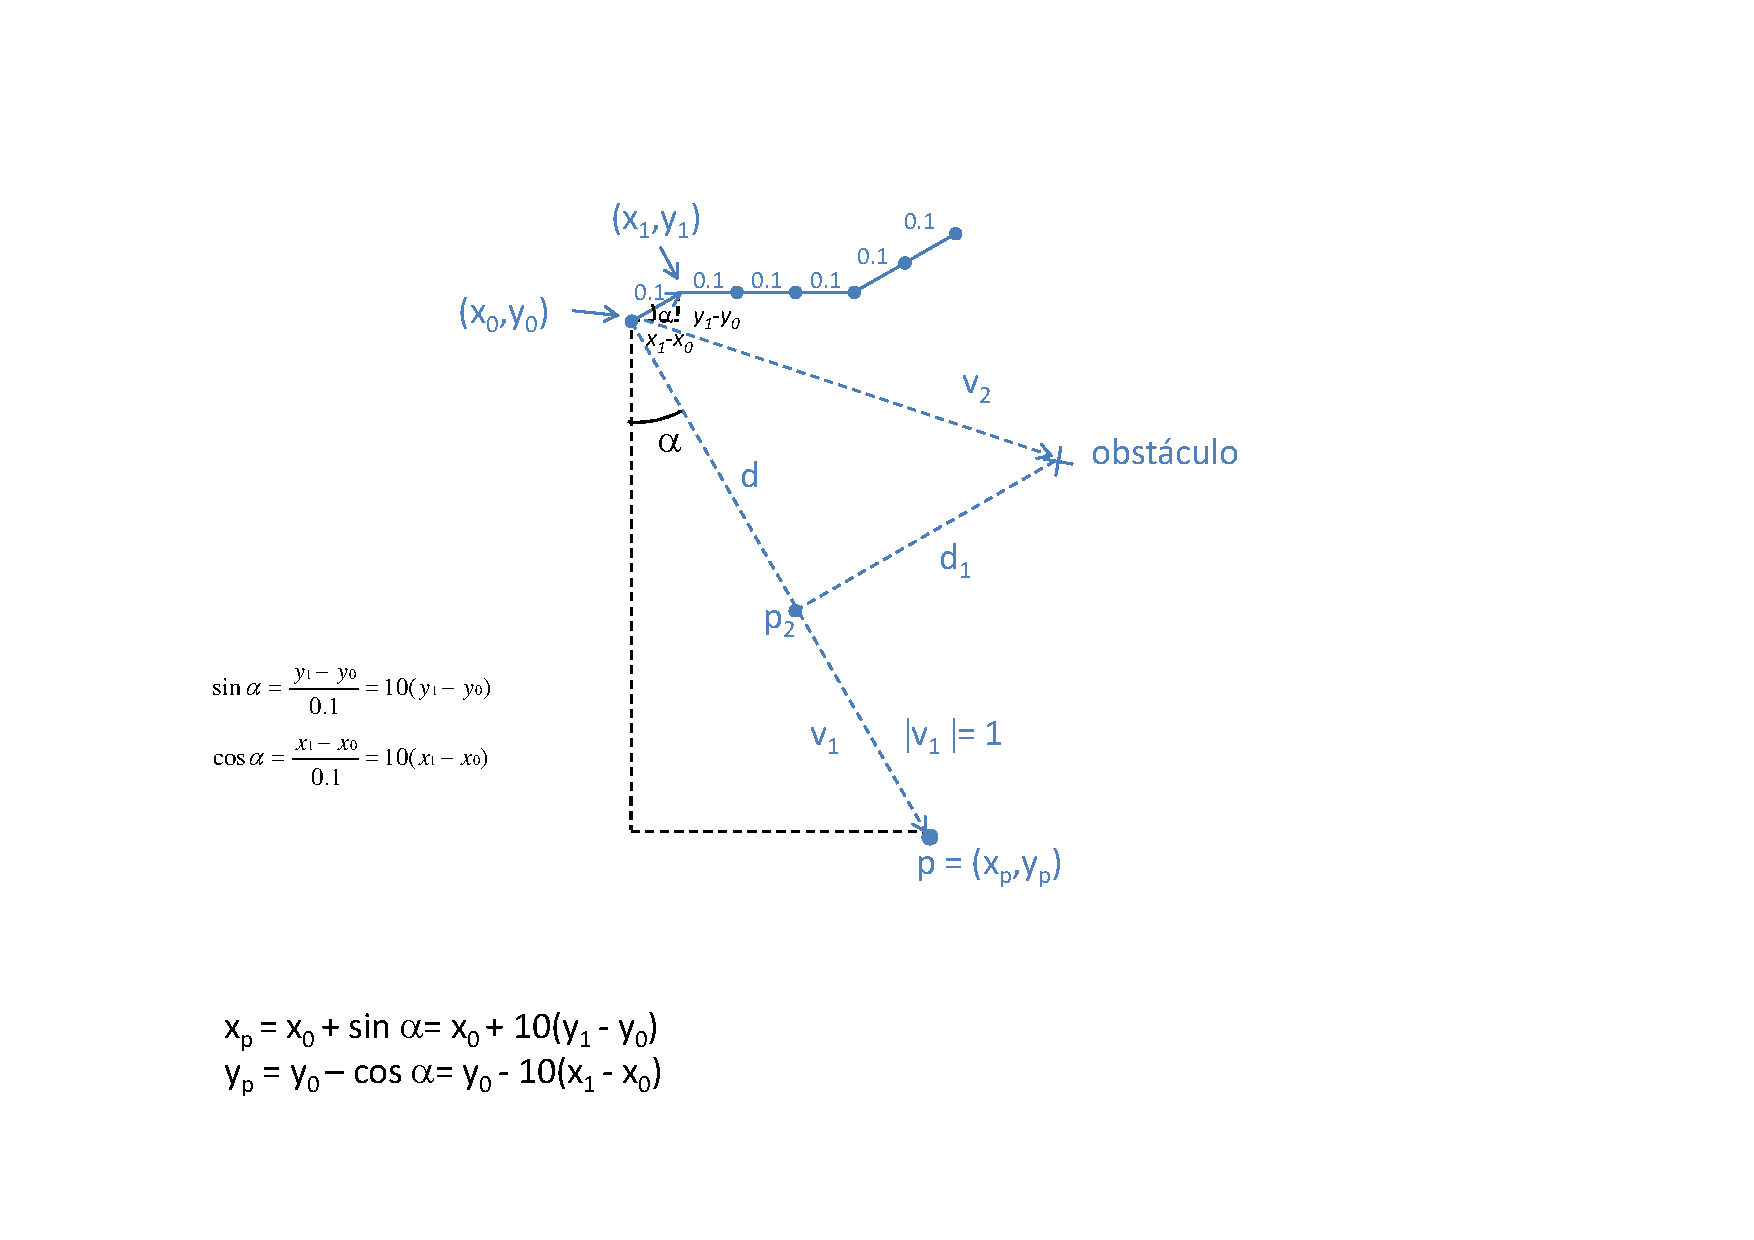
\includegraphics[scale=0.6]{elastic}\\
  \caption{Definición del punto $p$ y otras magnitudes para el punto de la trayectoria $i = 0$}\label{fg:elastic}
\end{figure}

%%%%%%%%%% pg 82 %%%%%%%%%%%%%%%%%%%%%%%%%%%%%

\pagebreak[4]
Se define un vector $v_{2}$ con origen en el punto de la trayectoria considerado y extremo los sucesivos puntos tomados como obstáculos. La proyección ortogonal de este vector sobre $v_{1}$ define un punto que llamaremos $p_{2}$. La distancia entre éste y el punto de la trayectoria se denota como $d$, que puede adoptar un signo u otro dependiendo de a qué lado de la trayectoria se encuentre el objeto. La distancia entre $p_{2}$ y el obstáculo correspondiente se mide mediante $d_{1}$.

En la deformación de la trayectoria sólo se utilizan los obstáculos que proporcionan un valor de $d_{1}$ suficientemente pequeño, puesto que la influencia de los objetos cercanos a tramos más avanzados de aquella podría llevar a malos resultados.

\begin{figure}[h]
  % Requires \usepackage{graphicx}
  \centering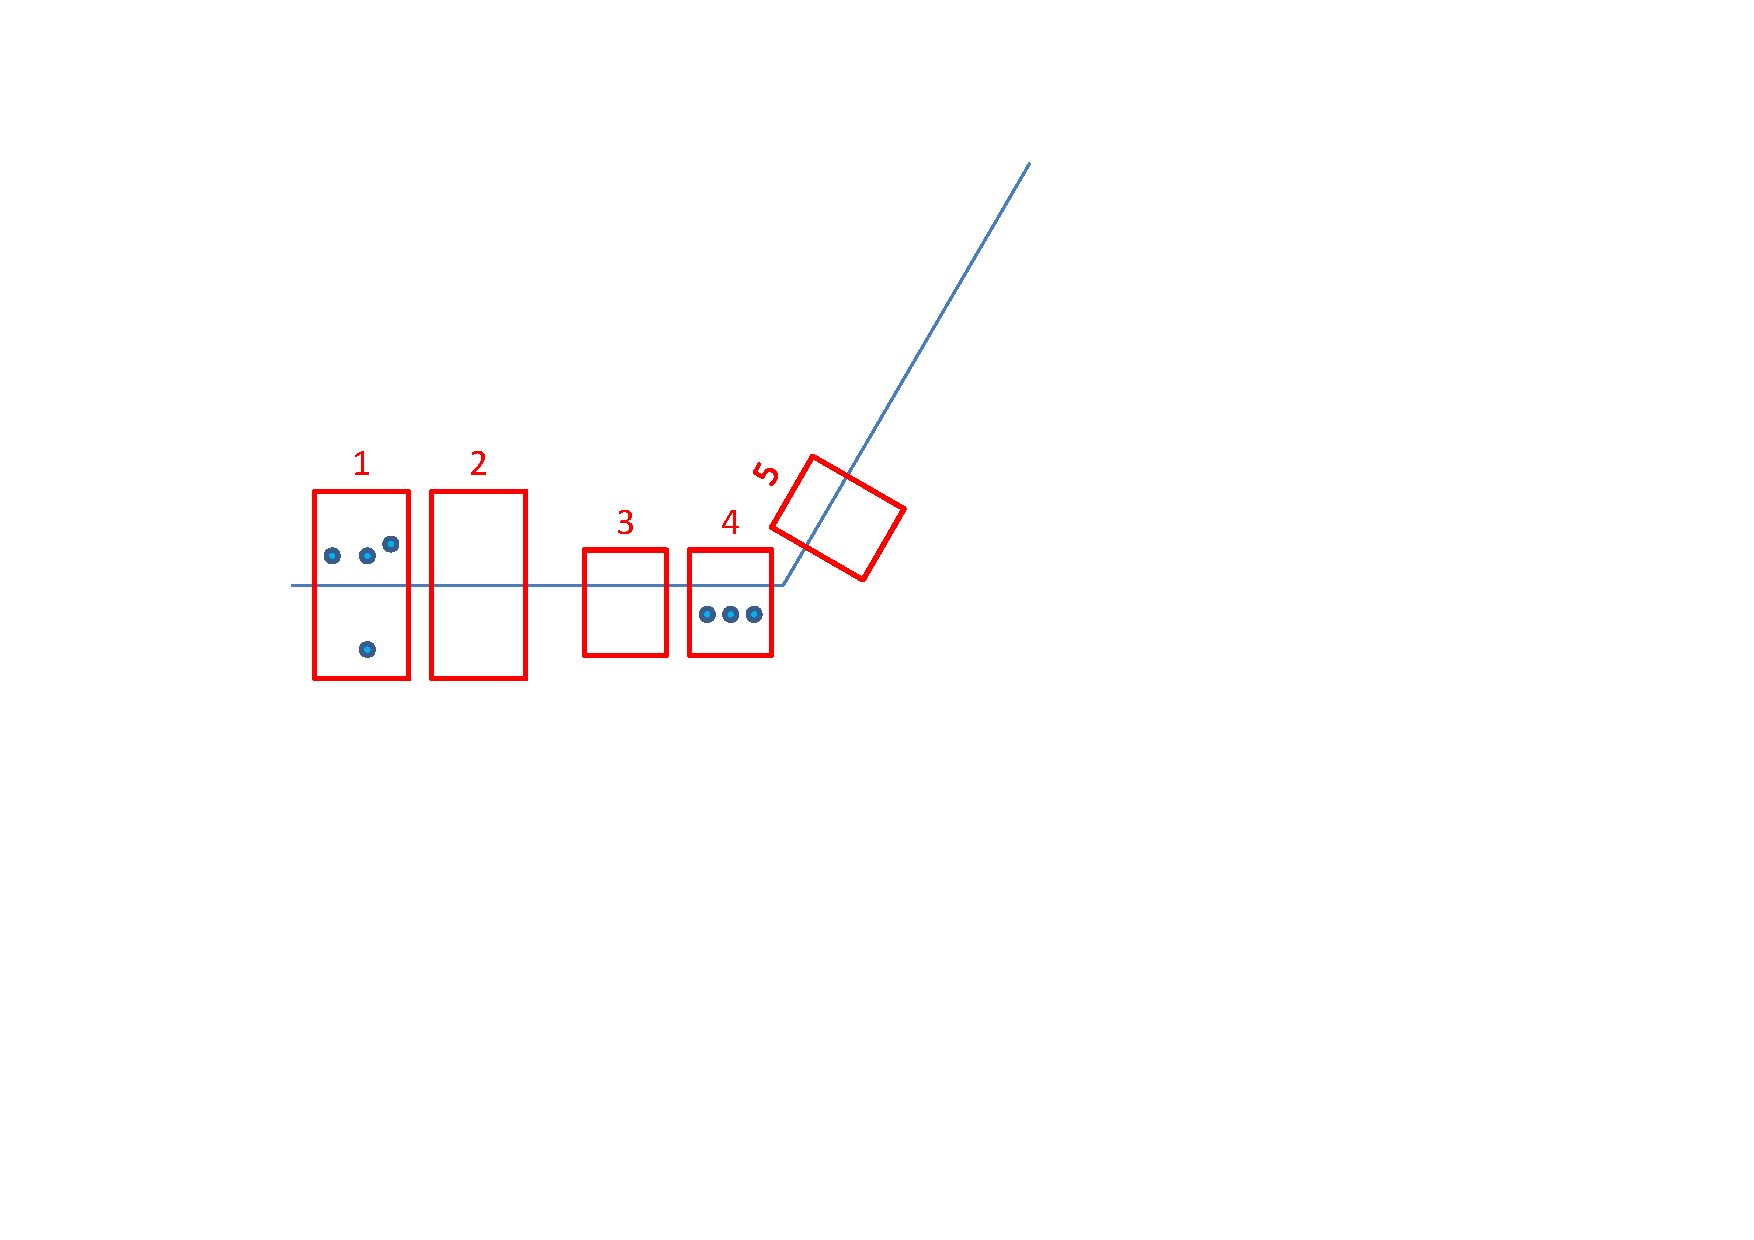
\includegraphics[scale=0.5]{d1}\\
  \caption{Los obstáculos del tramo 1 no deben afectar al 2 ni los del tramo 4 a los tramos 3 y 5.}\label{fg:d1}
\end{figure}

A través de un valor de $d$ corregido al tenerse en cuenta el radio del robot, se guardan para cada punto de la trayectoria las dos distancias mínimas a algún obstáculo a cada uno de los dos lados de la misma. Estas distancias se llamarán min\_int[i] y max\_int[i] respectivamente. Sus valores están inicializados con la máxima desviación que se le permite al robot, para el caso en que no haya ningún obstáculo en alguno de los lados y otras situaciones similares. Si después de recalcular dichos valores se cumple que min\_int $>$ max\_int, el robot no puede evitar los obstáculos sin superar la máxima desviación establecida y se dice que se encuentra en estado de bloqueo.

Haciendo la media entre esos dos valores se obtiene el desplazamiento, error [i], que debe aplicarse sobre el punto para que quede a la misma distancia de cada uno de los límites hallados para ambos lados (figura \ref{fg:elasticTray}).

\begin{figure}[h]
  % Requires \usepackage{graphicx}
  \centering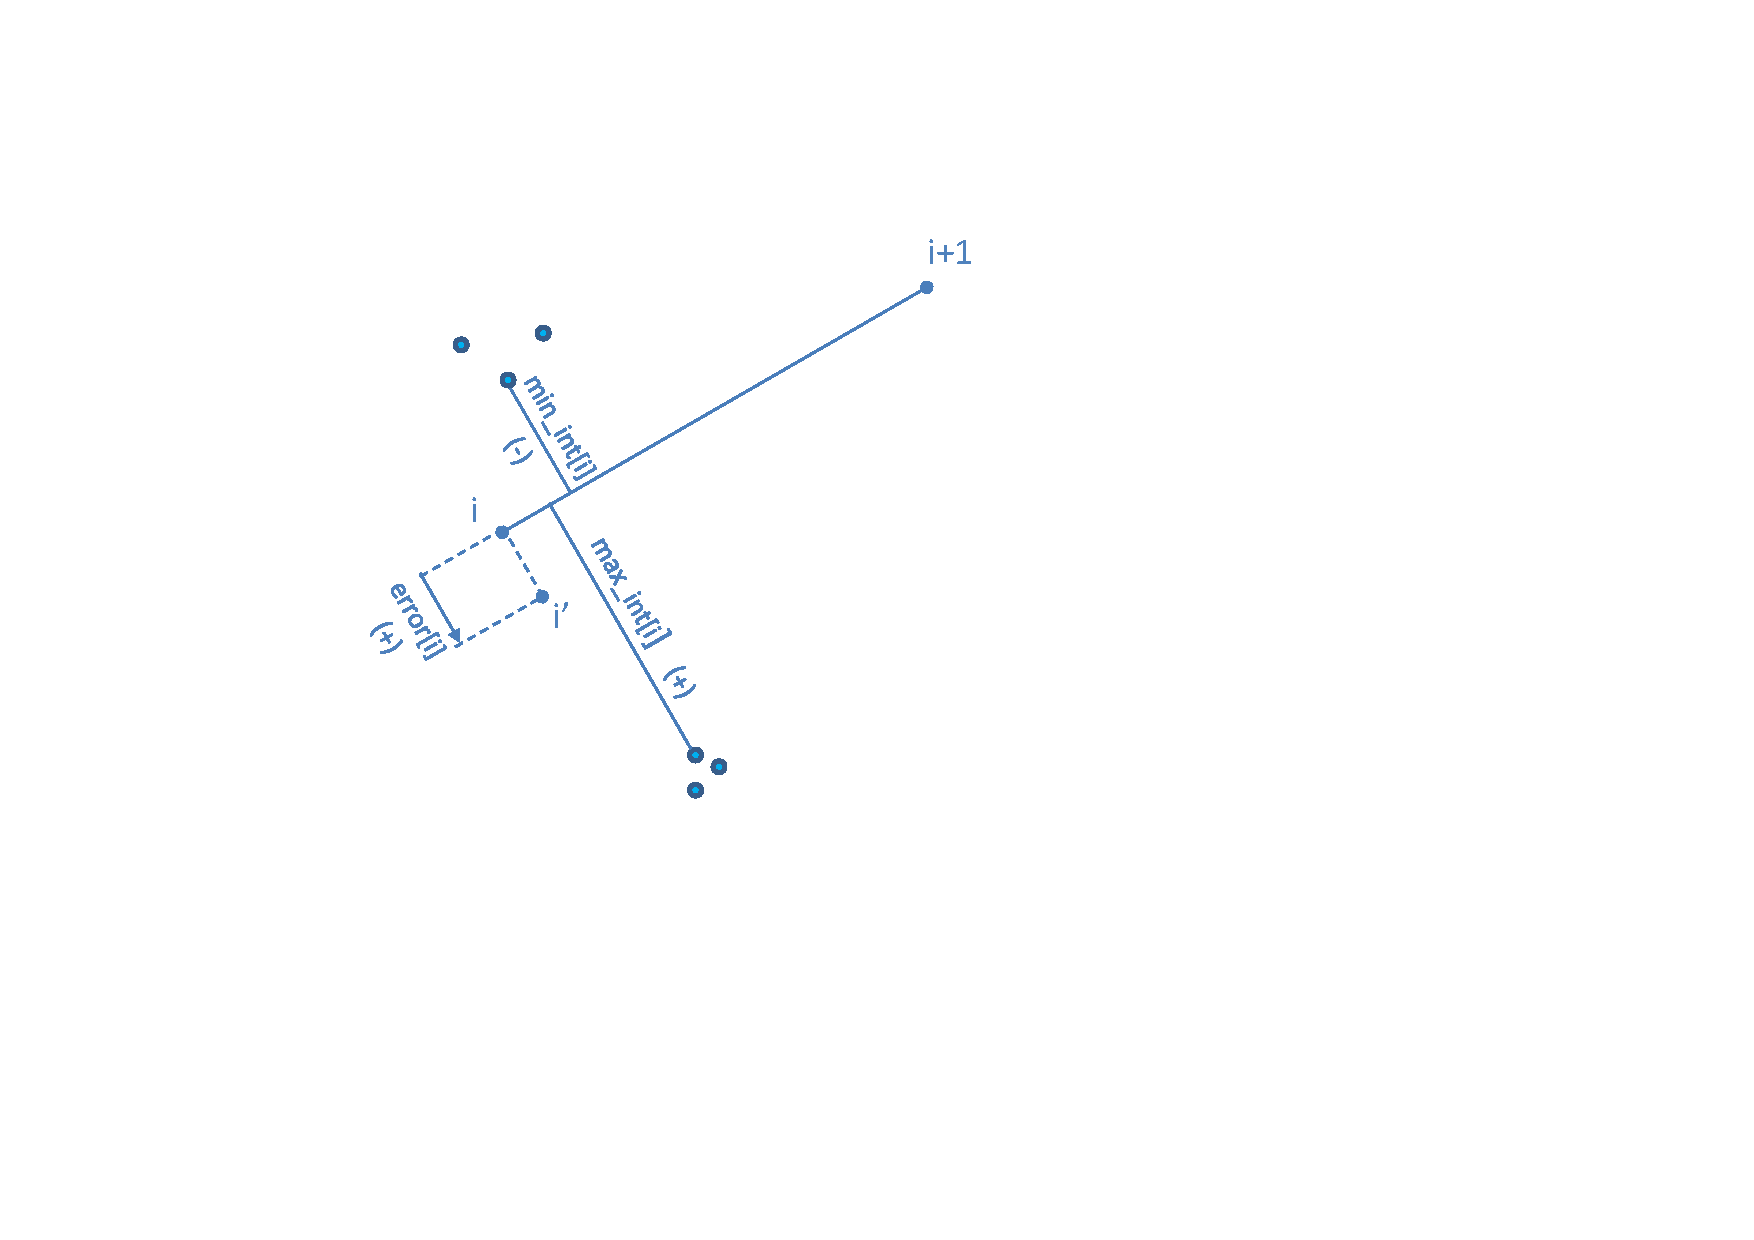
\includegraphics[scale=0.6]{elasticTray}\\
  \caption{Desplazamiento que sufre cada punto de la trayectoria}\label{fg:elasticTray}
\end{figure}

Con los puntos intermedios de la trayectoria lo que se hace es promediar el valor del error en el punto considerado con los valores del mismo en los puntos anterior y siguiente:

\begin{center}
$error2[i] = \frac{error[i-1] + error[i] + error[i+1]}{3}$
\end{center}

\noindent
De este modo se busca deformar la trayectoria más suavemente.

\section{La clase \prog{CMoveControl}}
En esta clase se llevan a cabo las tareas de control de movimiento, planificacón de trayectorias y control reactivo que se han descrito. Las principales funciones que se utilizan para ello son las siguientes:

\subsection{\prog{DefineDest}}

\noindent
\prog{void DefineDest(float x_d, float y_d, float tol)}

\noindent
Esta función sirve para definir el punto hacia el que tiene que dirigirse el robot.

\begin{itemize}
  \item \prog{x_d}: coordenada x del punto de destino.
  \item \prog{y_d}: coordenada y del punto de destino.
  \item \prog{tol}: distancia máxima al punto de destino para que se considere que éste ha sido alcanzado. Generalmente se utiliza una tolerancia de 50mm.
\end{itemize}

\noindent
Se guardan los argumentos en variables miembro, para que sus valores sean utilizados por el control de movimiento, y se establece el estado como \prog{NO_LLEGADO} mediante una macro con este nombre.

\subsection{\prog{Dist2Tray}}

\noindent
\prog{float Dist2Tray()}

\noindent
Esta función se utiliza para hallar la distancia del robot al segmento que une los puntos de la trayectoria entre los que se encuentra e indicar a qué lado del mismo está, de modo que pueda realizarse el control de acercamiento a la trayectoria descrito en \ref{control}.

\noindent
El cálculo de la distancia se lleva a cabo mediante los ángulos mostrados en la figura \ref{fg:dist2tray}, con la fórmula que aparece en ella. El valor que se devuelve es el de $d$.

\subsection{\prog{FindPoint}}

\noindent
\prog{int FindPoint()}

\noindent
Esta función se utiliza para ver cuál es el próximo punto de la trayectoria hacia el que debe ir el robot. Es útil en el caso de que haya pasado demasiado rápidamente por algún punto, para evitar que tenga que retroceder (ver última parte de \ref{control}).

\noindent
Se busca entre los cinco puntos de la trayectoria siguientes al de índice \prog{current_point} dentro del vector \prog{trajectory} aquel que esté más cerca del robot. Se devuelve el valor de su índice.

\subsection{\prog{GetCommand}}

\noindent
\prog{int GetCommand(float* vd, float* vs)}

\noindent
La función de este método consiste en calcular las velocidades de avance y giro con los que se va a mover el robot en cada momento. El paso de parámetros se realiza por referencia.

\begin{itemize}
  \item \prog{vd}: puntero a la velocidad de avance.
  \item \prog{vs}: puntero a la velocidad de giro.
\end{itemize}

\noindent
En primer lugar se mira si es necesario corregir el punto de destino con una llamada a la función \prog{FindPoint()} y si es así se hacen los correspondientes cambios. A continuación se determina el estado, viendo si la distancia entre la posición del robot y el punto de destino es menor que la tolerancia.

En la figura se muestra el diagrama de flujo simplificado de los pasos que se realizan a partir de este punto.

\begin{figure}[h]
  % Requires \usepackage{graphicx}
  \centering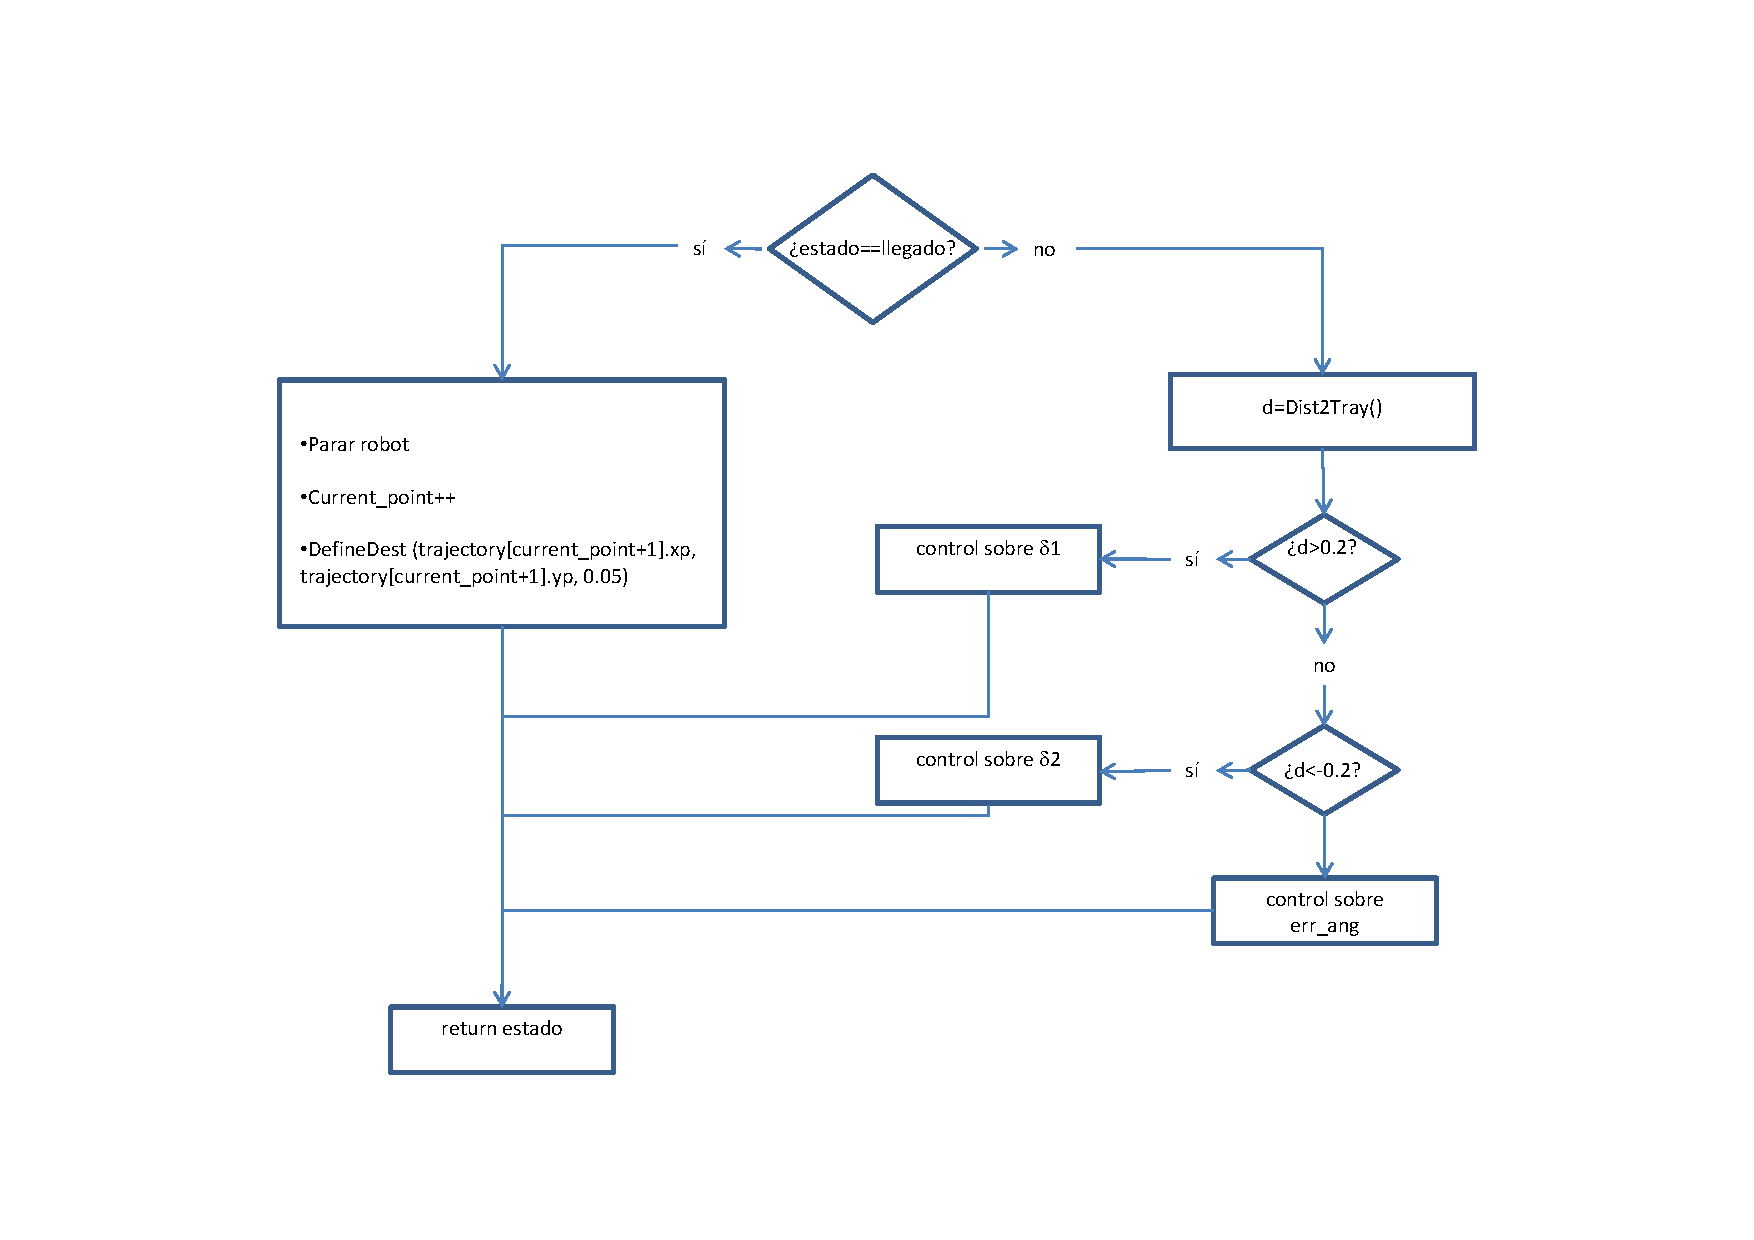
\includegraphics[scale=0.6]{flujo1}\\
  \caption{Diagrama de flujo simplificado de parte del proceso efectuado en \prog{GetCommand}}\label{fg:flujo1}
\end{figure}
Si el estado es \prog{NO_LLEGADO}, se determinan las velocidades mediante el procedimiento indicado en \ref{control} a partir de la posición del robot (disponible en toda la clase mediante las variables miembro \prog{x} e \prog{y}) y del punto guardado como destino.
Si el estado es \prog{LLEGADO} se da valor nulo a ambas velocidades y se incrementa una variable llamada \prog{current_point} que mide de este modo el índice del último punto de la trayectoria al que se ha llegado. Si efectivamente hay una trayectoria definida, se llama a la función \prog{DefineDest} para guardar como destino el siguiente punto de la misma (\prog{current_point + 1}). Los puntos de la trayectoria han de estar almacenados en un vector de la STL, vector \prog{trajectory}, miembro de la clase y definido para contener objetos CPoint2D.
\noindent
El valor de retorno es el estado.

\subsection{\prog{DefineTrajectory}}

\noindent
\prog{void DefineTrajectory(void)}

\noindent
Esta función se emplea para indicar que hay una trayectoria definida e inicializar el punto por el que debe empezarse a recorrerla (\prog{current_point = 0}).

\subsection{\prog{SmoothTrajectory}}

\noindent
\prog{std::vector<Point2D> SmoothTrajectory(float r)}

\noindent
Esta función se utiliza para suavizar la trayectoria.
\begin{itemize}
  \item \prog{r}: radio del arco con el que se suavizan los ángulos de la trayectoria.
\end{itemize}

\noindent
Los puntos de la trayectoria a suavizar se hallan guardados en un vector dinámico de nombre \prog{tray_prev} e inicialmente se copian en otro vector dínámico variable local de la función (vector \prog{smooth_tray}) para realizar en éste las modificaciones oportunas y no perder los puntos de la trayectoria original (de cara a la representación gráfica, principalmente).
Esta función es la implementación del algoritmo descrito en \ref{tray}. Se devuelve el vector \prog{smooth_tray}, que contiene los puntos de la trayectoria suave obtenida.

\subsection{\prog{ComputeElasticTray}}

\noindent
\prog{std::vector<Point2D> ComputeElasticTray()}

\noindent
Esta función sirve para deformar la trayectoria de forma que se aleje de los obstáculos (puntos 2D guardados en el vector de la STL \prog{v_puntos}, variable miembro de la clase).

\noindent
Los puntos de la trayectoria que se deforma son los almacenados en el vector \prog{nom_tray} de la STL, que se copian en una variable local de nombre \prog{ret_tray}. Con estos puntos se siguen los pasos indicados en el algoritmo de \ref{reactivo}. En caso de que al calcularse alguno de los nuevos puntos se produzca bloqueo (\prog{min_int[i] > max_int[i]}), se devuelve la trayectoria \prog{ret_tray} con los puntos hallados hasta ese momento. Si no se da situación de bloqueo, el vector \prog{ret_tray} se devuelve al final de la función y tendrá tantos puntos como la trayectoria inicial. El resultado de esta llamada será asignado al vector \prog{trajectory} para que pueda aplicarse el control de movimiento.

%\subsection{\prog{FindPoint}}
%
%\noindent
%\prog{int FindPoint()}
%
%\noindent
%Esta función se utiliza para ver cuál es el próximo punto de la trayectoria hacia el que debe ir el robot. Es útil en el caso de que haya pasado demasiado rápidamente por algún punto, para evitar que tenga que retroceder (ver última parte de \ref{control}).
%
%\noindent
%Se busca entre los cinco puntos de la trayectoria siguientes al de índice \prog{current_point} dentro del vector \prog{trajectory} aquel que esté más cerca del robot. Se devuelve el valor de su índice.

\subsection{\prog{DivideTrajectory}}

\noindent
\prog{int DivideTrajectory()}

\noindent
Esta función permite obtener una trayectoria igual a la inicial (\prog{nom_tray}) pero con el requisito de que cada uno de sus puntos no diste más de 0.1m del siguiente.


\noindent
Se utiliza un vector de la STL, variable local de la función, en el que se guarda cada punto de la trayectoria seguido de tantos otros puntos como sea necesario para que el segmento que va de aquél al próximo punto de \prog{nom_tray} cumpla la condición dada. El número de puntos intermedios que se añaden será $n = \frac{dist}{0.1} - 1$, siendo $dist$ la longitud del segmento inicial. Finalmente se iguala el vector \prog{nom_tray} al vector con los nuevos puntos.

\begin{figure}[h]
  % Requires \usepackage{graphicx}
  \centering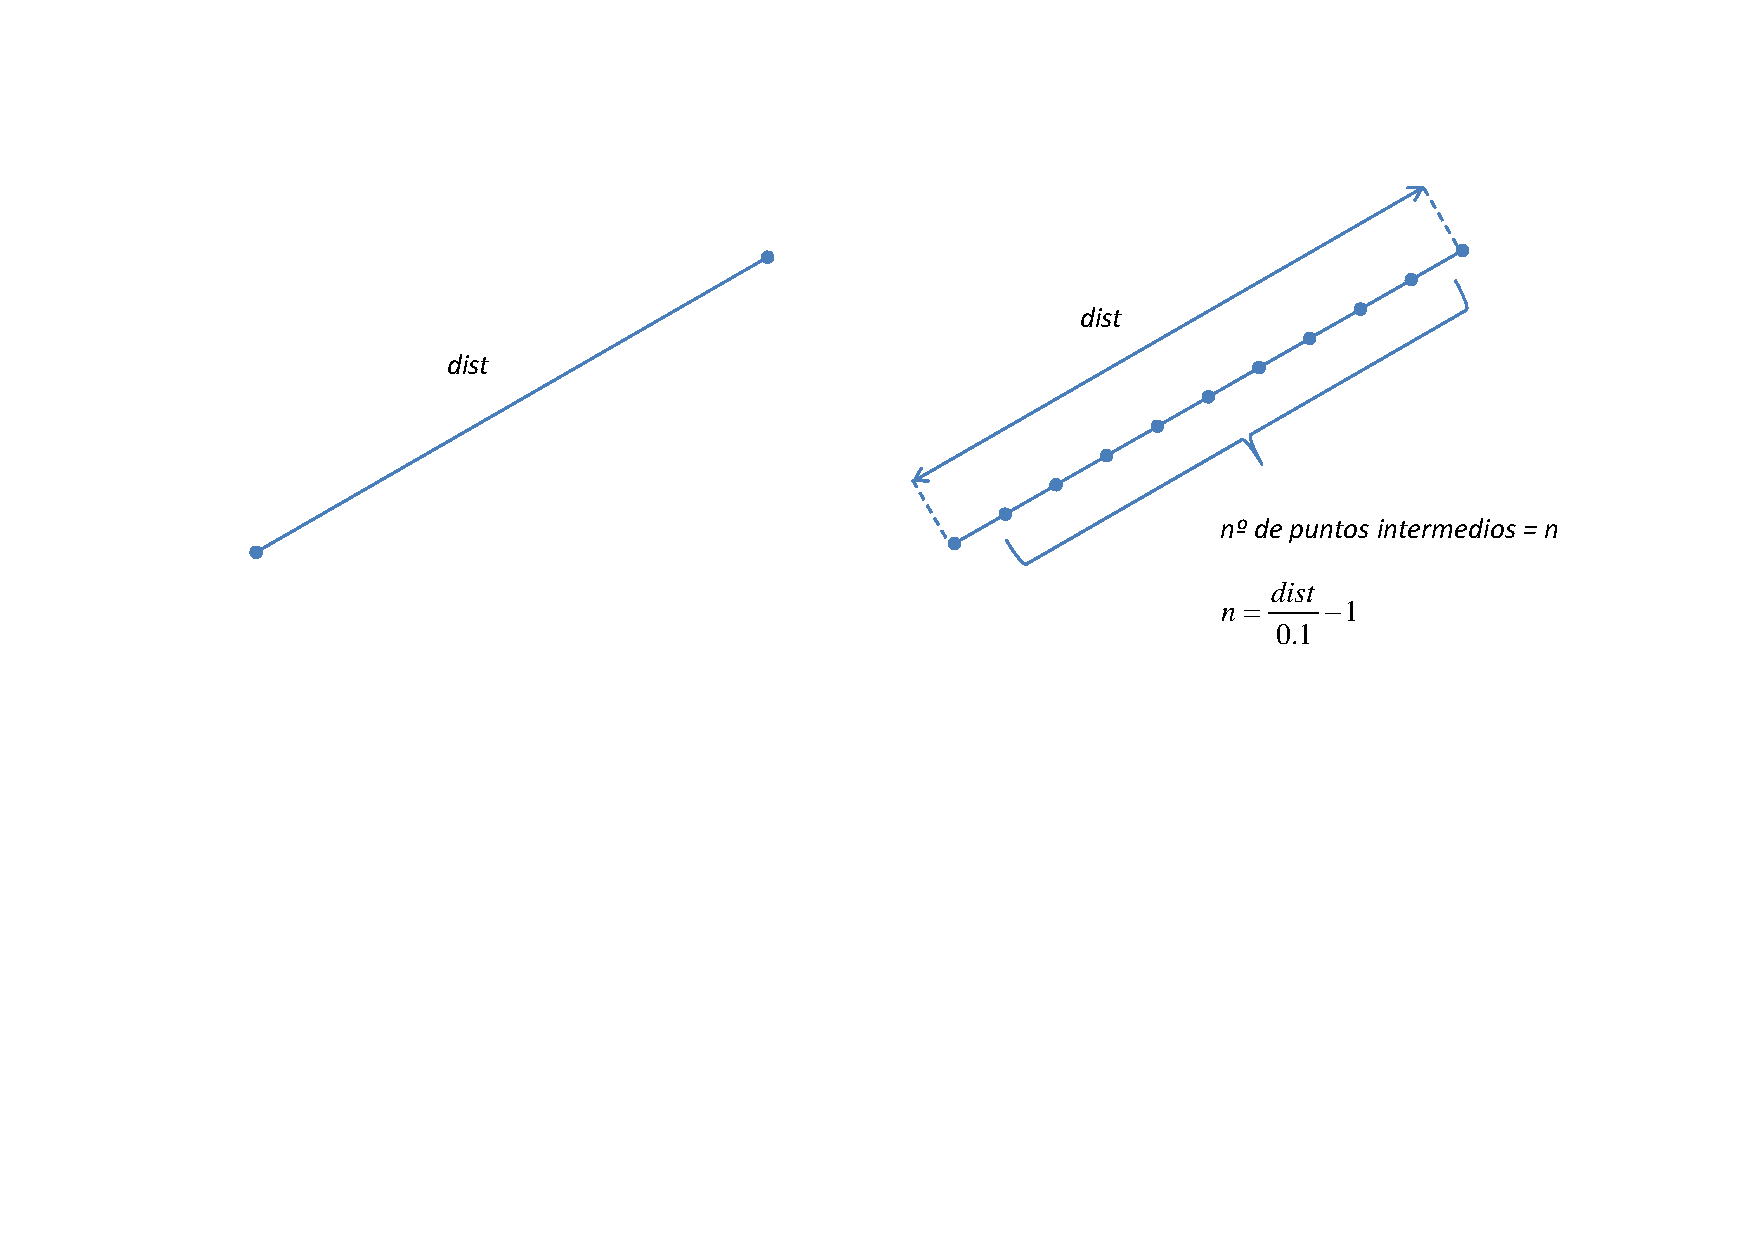
\includegraphics[scale=0.6]{divide}\\
  \caption{Puntos de un segmento de la trayectoria original y del resultado de la llamada a \prog{DivideTrajectory()}}\label{fg:divide}
\end{figure}

\vspace{0.2cm}

\noindent
La utilidad de esta función reside en la necesidad de tener los puntos de la trayectoria suficientemente juntos para que el control reactivo que se implementa a través de \prog{ComputeElasticTray()} sea efectivo. Si no fuera así, el filtro que se realiza mediante $d_{1}$ no permitiría esquivar muchos de los obstáculos.

%\subsection{\prog{Dist2Tray}}
%
%\noindent
%\prog{float Dist2Tray()}
%
%\noindent
%Esta función se utiliza para hallar la distancia del robot al segmento que une los puntos de la trayectoria entre los que se encuentra e indicar a qué lado del mismo está, de modo que pueda realizarse el control de acercamiento a la trayectoria descrito en \ref{control}.
%
%\noindent
%El cálculo de la distancia se lleva a cabo mediante los ángulos mostrados en la figura \ref{fg:dist2tray}, con la fórmula que aparece en ella. El valor que se devuelve es el de $d$.


\section{Pruebas y resultados}
Todas las funcionalidades de control de movimiento, planificación de trayectorias y control reactivo del proyecto han sido probadas inicialmente mediante simulación gráfica. Esto permite la depuración y mejora del comportamiento del programa de una forma más cómoda. Las pruebas con robots reales requieren más espacio y pueden conllevar mayores riesgos si no se han llevado a cabo previamente en simulación. Además, es preciso cargar baterías, llevar el ejecutable al ordenador portátil que se utiliza, realizar la conexión \emph{telnet} e introducir las contraseñas correspondientes\ldots por lo que resultan bastante más lentas. El control de movimiento, sin embargo, sí que fue probado en modo real en fases anteriores del proyecto ya que la respuesta del robot ante las velocidades aplicadas puede ser algo diferente en uno y otro caso y resultaba conveniente ajustar bien los parámetros para no seguir trabajando con un regulador inadecuado.

\subsection{Pruebas en modo \emph{simulación}}

\subsubsection{Control de movimiento y planificación de trayectorias}

\noindent
\textbf{\textbf{1.} Seguimiento de una trayectoria planificada a priori}

En este caso, lo que se ha hecho es definir los puntos de la trayectoria inicial mediante doble click con el botón derecho del ratón sobre la interfaz gráfica. Según se van añadiendo puntos se va suavizando la trayectoria. Cuando se ha completado la definición de la trayectoria deseada se indica que el robot debe seguirla y éste comienza a moverse sobre la misma. En la figura puede verse en color azul la trayectoria resultante tras la planificación, en verde la trayectoria seguida de acuerdo con las medidas de la odometría y en rojo la trayectoria seguida según la localización. Como las medidas del láser en modo simulación se hallan a 8000m del robot (ver método \prog{Simulate}, de \ref{CPosData}), no se realiza asociación de datos ni se corrige la posición, de modo que las trayectorias dibujadas en verde y rojo serán necesariamente iguales. La única diferencia reside en el hecho de que se han representado a diferentes alturas.


\textbf{Resultados:}
\begin{figure}[h]
  % Requires \usepackage{graphicx}
  \centering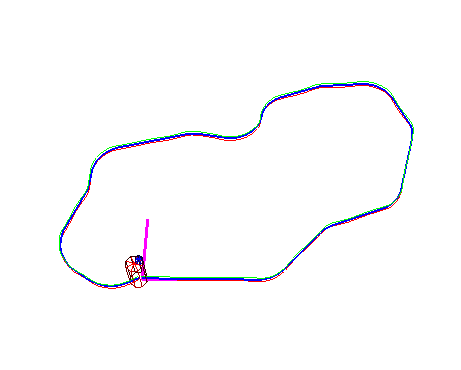
\includegraphics[scale=0.4]{mov1}\\
  \caption{Primer experimento de planificación de trayectorias y control de movimiento}\label{fg:mov1}
\end{figure}

Como puede verse, la trayectoria seguida por el robot es prácticamente idéntica a la planificada, lo que muestra el buen diseño del controlador.

\noindent
\textbf{\textbf{2.} Seguimiento de una trayectoria planificada a priori con el robot Pioneer P3AT}

Esta es una de las pruebas que se realizó con el control elaborado para el robot Pioneer P3AT de MobileRobots/Activmedia. En ella se utiliza MobileSim, un software de simulación proporcionado por los fabricantes para la experimentación con Aria. MobileSim está construido sobre el simulador Stage (creado por Richard Vaughan, Andrew Howard y otros como parte del proyecto Player/Stage), con algunas modificaciones por parte de MobileRobots. Utilizando la clase \prog{SimpleConnector} de la biblioteca Aria, la conexión se inicia por defecto con el simulador.


\textbf{Resultados:}
\begin{figure}[h]
  % Requires \usepackage{graphicx}
  \centering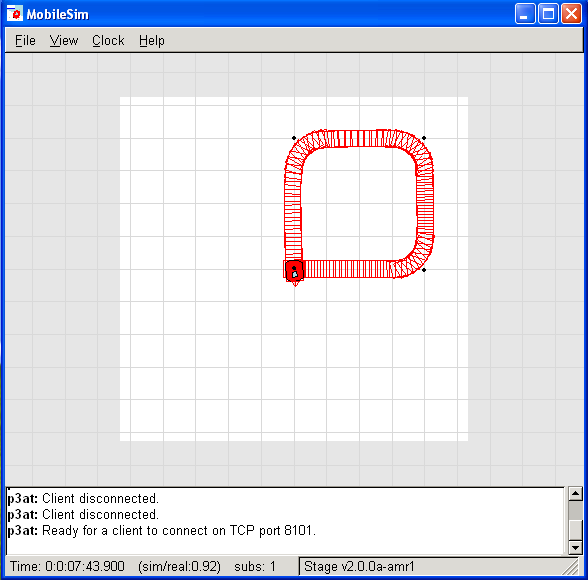
\includegraphics[scale=0.4]{mov2}\\
  \caption{Segundo experimento de planificación de trayectorias y control de movimiento}\label{fg:mov2}
\end{figure}

La trayectoria inicial definida en este caso es la formada por los puntos marcados en negro. Puede observarse que el control proporciona de nuevo un buen resultado.

\noindent
\textbf{\textbf{3.} Seguimiento de una trayectoria planificada dinámicamente}

En esta prueba se generan nuevos puntos de la trayectoria a medida que el robot se acerca a su próximo destino. En algunos casos, al llegar el robot a un punto y posteriormente añadir otro punto después de aquél, el algoritmo que suaviza la trayectoria hace que ésta deje de pasar por el punto en el que se encontraba el robot. Si se produce esta circunstancia, entra en acción el controlador para evitar desvíos sobre la trayectoria planificada. El buen funcionamiento del mismo puede verse con claridad en las figuras \ref{fg:mov3} y \ref{fg:mov4}:



\textbf{Resultados:}
\begin{figure}[h]
  % Requires \usepackage{graphicx}
  \centering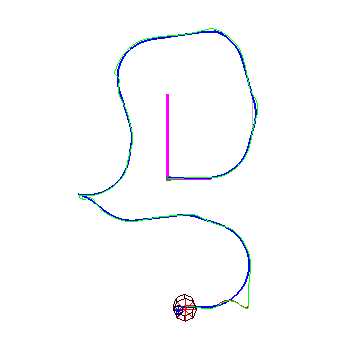
\includegraphics[scale=0.4]{mov3}\\
  \vspace{2cm}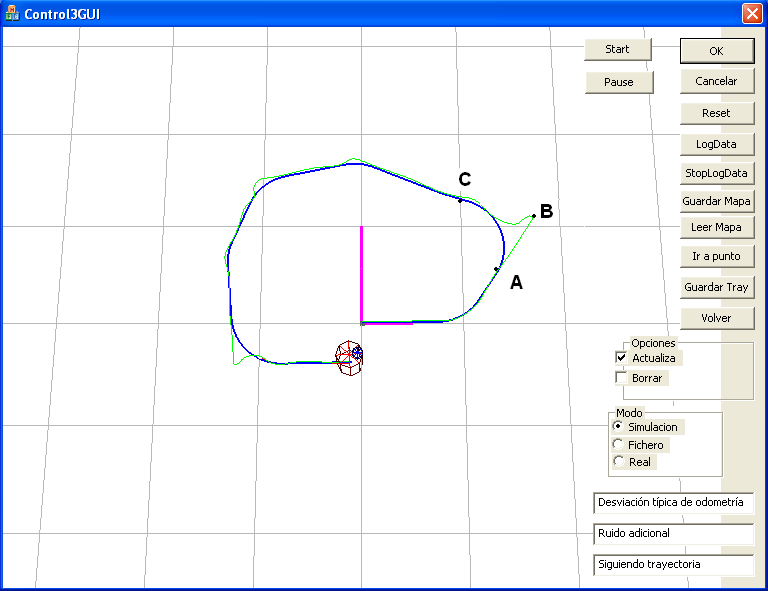
\includegraphics[scale=0.4]{mov_3}
  \caption{Tercer experimento de planificación de trayectorias y control de movimiento}\label{fg:mov3}
\end{figure}


En la segunda figura, por ejemplo, el robot llega al punto B procedente del A y, seguidamente, se añade a la trayectoria el punto C. El algoritmo para suavizar trayectorias redondea entonces la trayectoria que habría de estar formada por A, B y C, pero el robot ya se encuentra en B. El regulador inicial conduciría al robot directamente hacia C pero las mejoras introducidas hacen que el robot se aproxime primero a la trayectoria planificada.

\noindent
\textbf{\textbf{4.} Seguimiento del camino de vuelta después de que el robot ejecute una trayectoria.}

En este caso, se define una trayectoria mediante el ratón o moviendo al robot por teleoperación con el teclado (sección \ref{opciones}). Cuando finaliza el seguimiento de la misma, el robot es capaz de regresar de forma autónoma al punto de partida si así se le indica. En la primera figura que se muestra, la trayectoria inicial está definida mediante el ratón mientras que en la segunda se utiliza el modo teleoperado. La trayectoria dibujada en color verde es la correspondiente a la odometría durante la ida y la que aparece en rosa es la odometría del camino de vuelta.

\textbf{Resultados:}
\begin{figure}[h]
  % Requires \usepackage{graphicx}
  \centering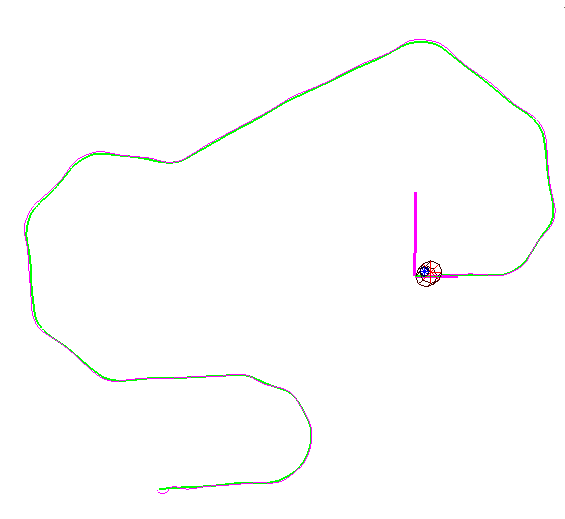
\includegraphics[scale=0.4]{vuelta}\\
  \hspace{0.5cm}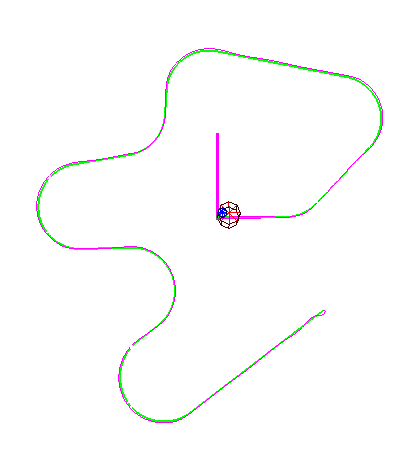
\includegraphics[scale=0.4]{vuelta2}
  \caption{Cuarto experimento de planificación de trayectorias y control de movimiento}\label{fg:mov4}
\end{figure}


\subsubsection{Control reactivo}

\noindent
\textbf{\textbf{1.} Obtención de trayectorias deformadas ante la presencia de obstáculos cercanos a una trayectoria definida}
En esta prueba se define primeramente una trayectoria y a continuación se crean obstáculos más o menos cercanos a la misma mediante doble click con el botón izquierdo del ratón sobre el punto en el que debe situarse cada uno de ellos. En el momento en que se añade un obstáculo, la trayectoria se deforma mediante el algoritmo previamente explicado. En este caso no se han incorporado obstáculos nuevos durante el movimiento del robot sobre la trayectoria, por lo que no se trata de una aplicación de control reactivo sino sólo de una prueba del algoritmo de deformación.

\textbf{Resultados:}
\begin{figure}[h]
  % Requires \usepackage{graphicx}
  \centering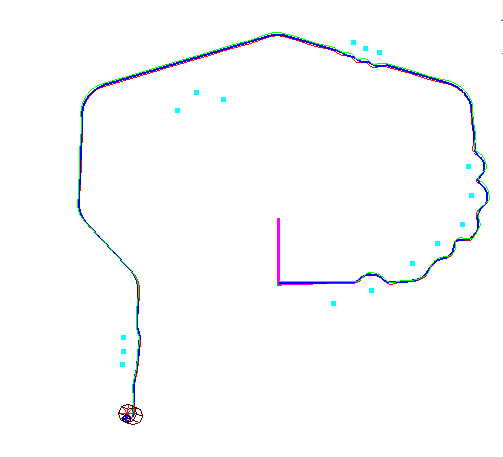
\includegraphics[scale=0.4]{obs2}\\
  \hspace{0.5cm}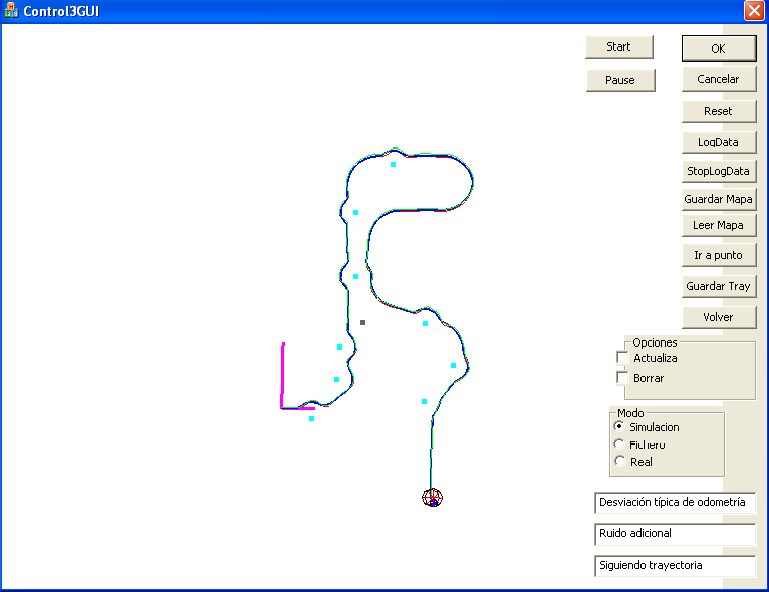
\includegraphics[scale=0.4]{obs3}
  \caption{Experimento previo para el control reactivo}\label{fg:react1}
\end{figure}


Como puede verse, los obstáculos se han representado en color cyan. La trayectoria se deforma de un modo suave en los puntos cercanos a ellos sin superar la máxima desviación permitida, establecida en 0.15m. Los obstáculos suficientemente alejados de la trayectoria no suponen ninguna modificación en la misma. En la segunda figura hay un obstáculo que afecta a dos tramos diferentes de la trayectoria y ambas deformaciones se realizan correctamente. Con este valor de la máxima desviación permitida no pueden esquivarse obstáculos que se encuentren sobre la trayectoria a seguir. En este caso, para el robot Urbano, entrarían en acción los mecanismos de control reactivo de bajo nivel (comandos de parada y giro). Si se utiliza en su lugar un valor de 0.6m, las deformaciones son mayores y pueden evitarse los obstáculos que supondrían un choque directo (figura \ref{react2}). El problema que conlleva esta opción es que en el caso de entornos densos (como son la mayoría de los entornos de interiores), las deformaciones son excesivas hacia uno y otro lado y se pierde suavidad en la trayectoria.
\begin{figure}[h]
  % Requires \usepackage{graphicx}
  \centering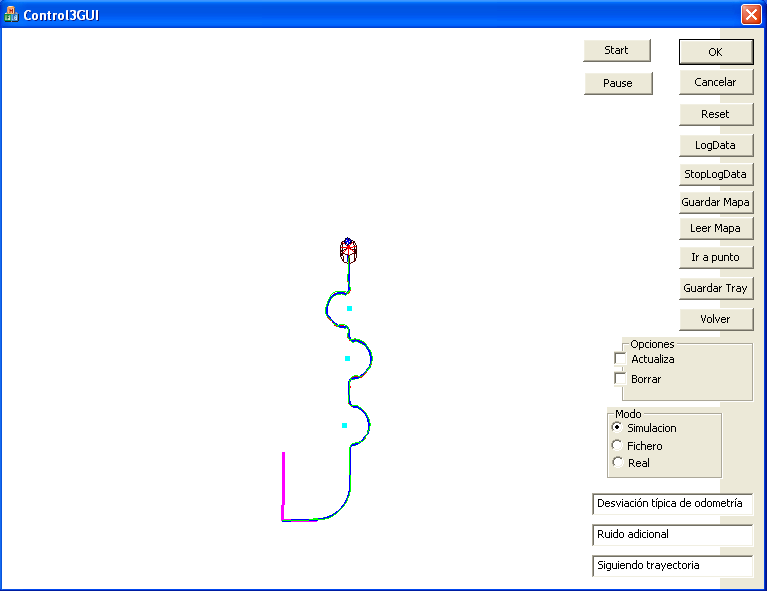
\includegraphics[scale=0.4]{obs4}\\
  \caption{Aumento de la máxima desviación permitida}\label{fg:react2}
\end{figure}


\noindent
\textbf{\textbf{2.} Trayectoria seguida por el robot ante la aparición de un obstáculo durante su movimiento sobre una trayectoria}

En este caso se ha llevado el robot a un punto por medio de una trayectoria definida sobre la interfaz gráfica y se le ha indicado que regrese a su posición inicial. Durante el camino de vuelta, se ha creado un obstáculo en la trayectoria teórica que debería seguir el robot para ver su respuesta simulada en tiempo real.

\textbf{Resultados:}
En la figura \ref{fg:react3} se ha plasmado en color verde la trayectoria seguida por el robot durante la ida (trayectoria teórica de vuelta) y en colores azul y magenta la trayectoria real efectuada ante la presencia del obstáculo.
\begin{figure}[h]
  % Requires \usepackage{graphicx}
  \centering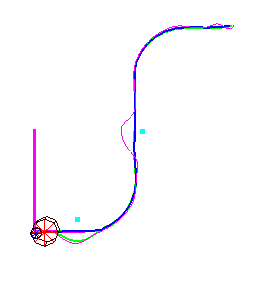
\includegraphics[scale=0.4]{react2}\\
  \caption{Primer experimento de control reactivo}\label{fg:react3}
\end{figure}


\subsection{Pruebas en modo \emph{real}}
Cuando se utiliza el sistema con el robot real las llamadas a \prog{GetCommand} se realizan cada 300ms aproximadamente. Como se verá en los siguientes resultados, el seguimiento de la trayectoria es algo menos preciso que en las pruebas realizadas en simulación.

\subsubsection{Control de movimiento y planificación de trayectorias}

\noindent
\textbf{\textbf{1.} Seguimiento de una trayectoria planificada a priori}
En estas pruebas lo que se ha hecho es definir una trayectoria con el ratón, al igual que en el modo simulación, y ver cómo el robot se va dirigiendo hacia los correspondientes puntos de la misma. La longitud de las trayectorias efectuadas está limitada por el entorno de experimentación, una zona del laboratorio no muy amplia y con objetos cercanos que disminuyen el área explorable.

\textbf{Resultados:}
En la figura \ref{fg:real1} se muestra en color azul la trayectoria nominal seleccionada y en colores verde y rojo la seguida por el robot.
\begin{figure}[h]
  % Requires \usepackage{graphicx}
  \centering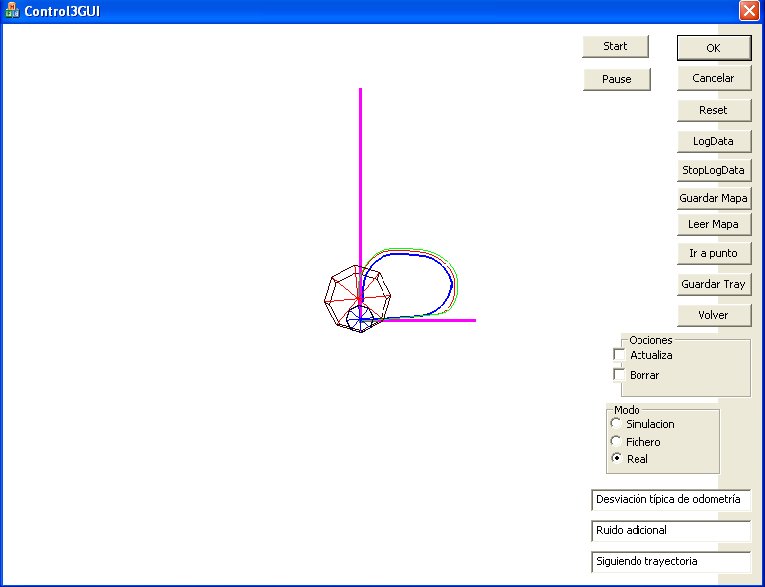
\includegraphics[scale=0.4]{real}\\
  \hspace{0.5cm}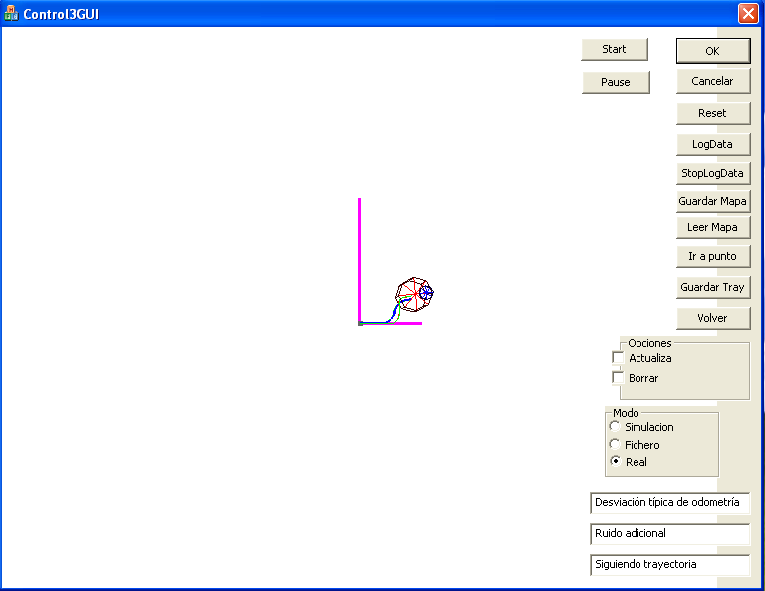
\includegraphics[scale=0.4]{real1}
  \caption{Primer experimento de movimiento con robot real}\label{fg:real}
\end{figure}

En el segundo caso se aprecia que el mantenimiento de la dirección de la trayectoria prevalece frente a la acción de acercar el robot a la misma, pero esto evita que la trayectoria resultante sea más ondulada.

\noindent
\textbf{\textbf{2.} Seguimiento del camino de vuelta después de que el robot ejecute una trayectoria.}
La forma de proceder en este caso es la misma que en el modo de simulación.
\textbf{Resultados:}
En la figura \ref{fg:real2} se muestra en color verde la trayectoria durante la ida y en color rosa la correspondiente al camino de vuelta.
\begin{figure}[h]
  % Requires \usepackage{graphicx}
  \centering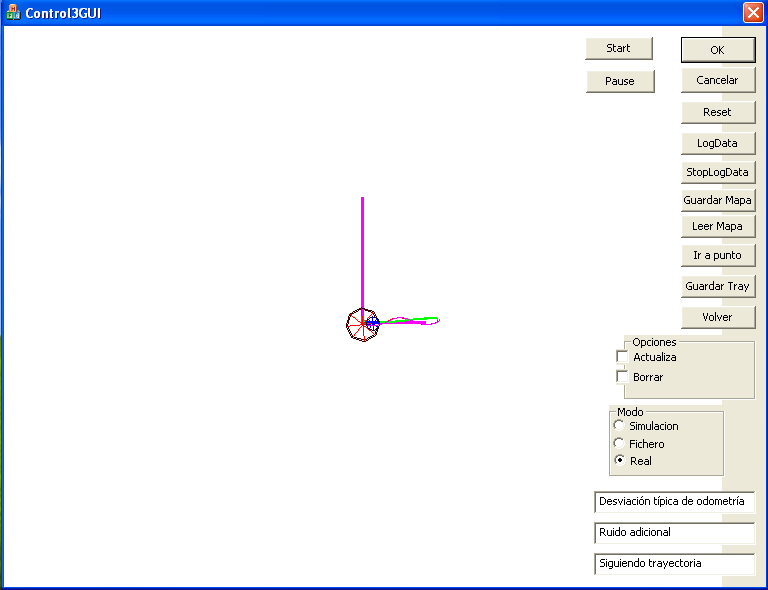
\includegraphics[scale=0.4]{real2}\\
  \caption{Segundo experimento de movimiento con robot real}\label{fg:real2}
\end{figure}

Como puede observarse, en este caso aparecen mayores desviaciones respecto a la trayectoria definida. La desviación producida al dar la vuelta el robot hace que éste tarde un poco en coger la dirección correcta, pero las acciones de control sobre err\_ang2 y err\_ang3 permiten que los cambios no sean demasiado bruscos. Si la trayectoria fuera más larga podría verse que la estabilización es bastante rápida.
